\documentclass[12pt, letterpaper]{template}
\usepackage[numbers]{natbib} % or [authoryear]
\usepackage{amsmath}
\usepackage[ruled,vlined,linesnumbered]{algorithm2e}
\usepackage{placeins}
\bibliographystyle{plainnat}
\usepackage{subcaption}
\usepackage{float}
\usepackage{tabularx}
\usepackage{amsthm}
\newtheorem{lemma}{Lemma}

\hypersetup{
    colorlinks=true,
    citecolor=blue,
    linkcolor=blue,
    urlcolor=black
}

\definecolor{darkblue}{rgb}{0, 0, 0.5}

\usepackage{url}            % simple URL typesetting
\urlstyle{same}  % makes URLs use the same font as normal text
\usepackage{booktabs}       % professional-quality tables
\usepackage{amsfonts}       % blackboard math symbols
\usepackage{nicefrac}       % compact symbols for 1/2, etc.
\usepackage{microtype}      % microtypography
\usepackage{xcolor}         % colors
\usepackage{abstract}       
\usepackage{tikz}
\usepackage{pgfplots, pgfplotstable}
\pgfplotsset{compat=1.15}

\usepackage{lineno}

\usepackage{enumitem}       % [leftmargin=20pt]
\usepackage{subfig}         % subfloat
\usepackage{graphicx}
\let\originalincludegraphics\includegraphics
\renewcommand{\includegraphics}[2][]{%
  \IfFileExists{#2}{%
    \originalincludegraphics[#1]{#2}%
  }{%
    \fbox{%
      \begin{minipage}[c][0.18\textheight][c]{0.8\linewidth}
        \centering
        Missing figure:\\
        \texttt{\detokenize{#2}}
      \end{minipage}%
    }%
  }%
}
\usepackage{multirow}       %
\usepackage{xspace}         % xspace
\usepackage{wrapfig}        % wrapfigure
\usepackage{colortbl}
\usepackage{bbm}            % indicator function (\mathbbm)
\usepackage{adjustbox}
\usepackage{xcolor}
\usepackage{tocloft}

% Put the word "Figure" / "Table" before the number in the lists
\renewcommand{\cftfigpresnum}{Figure\ }
\renewcommand{\cfttabpresnum}{Table\ }

% Set the width reserved for "Figure <num>" and "Table <num>"
% Tune these lengths until wrapping aligns nicely.
\setlength{\cftfignumwidth}{4.5em}
\setlength{\cfttabnumwidth}{4.5em}

\usepackage[utf8]{inputenc}
\usepackage{lmodern}
\usepackage{makecell}
\usepackage{utfsym}
\usepackage{xcolor}
% \usepackage{hyperref}
\usepackage{multirow}

\providecommand{\keywords}[1]
{
  \small	
  \textbf{Keywords:} #1
}

\usepackage[most,skins,theorems]{tcolorbox}
\tcbset{
  aibox/.style={
    width=\linewidth,
    top=8pt,
    bottom=4pt,
    colback=blue!6!white,
    colframe=black,
    colbacktitle=black,
    enhanced,
    center,
    attach boxed title to top left={yshift=-0.1in,xshift=0.15in},
    boxed title style={boxrule=0pt,colframe=white,},
  }
}
\newtcolorbox{AIbox}[2][]{aibox,title=#2,#1}

\setlength\parindent{0pt}
\setcounter{tocdepth}{3}

% My commands
\newcommand{\tabitem}{\textbullet~~}

\newcommand{\PRM}{PRM\xspace}
\newcommand{\minprev}{\mathit{minprev}}

\theoremstyle{definition}
\newtheorem{definition}{Definition}[section]
\newtheorem{property}[definition]{Property}
\newtheorem{remark}[definition]{Remark}

\newcommand{\specialcell}[2][c]{\begin{tabular}[#1]{@{}c@{}}#2\end{tabular}}
\newcommand{\official}{$^{*}$}
\newcommand{\tms}{$\times$}
\newcommand{\mean}[1]{#1}
\newcommand{\bmean}[1]{\textbf{#1}}
\newcommand{\improve}[1]{\scalebox{.70}{\color{red!50!black}#1}}
\newcommand{\std}[1]{\scalebox{.70}{$\pm$ #1}}
\newcommand{\bstd}[1]{\scalebox{.70}{\textbf{$\pm$ #1}}}
\newcommand{\revise}[1]{{\color{magenta}[#1]}}

\newcommand{\mycolor}{cyan!10}
\newcommand{\highlight}{\cellcolor{\mycolor}}

\newcommand{\cmark}{\ding{51}}
\newcommand{\xmark}{\ding{55}}

\newcommand\blfootnote[1]{%
  \begingroup
  \renewcommand\thefootnote{}\footnote{#1}%
  \addtocounter{footnote}{-1}%
  \endgroup
}


\title{}


\newcommand{\fix}{\marginpar{FIX}}
\newcommand{\new}{\marginpar{NEW}}


\begin{document}

\begin{titlepage}

\center % Center everything on the page


\includegraphics[width=12cm]{figures/FPTU_logo.png}\\[1cm] 
%\includegraphics[width=12cm]{title/black-stacked-trinity.jpg}\\[1cm] 

\Large FPT University\\[1.5cm] % Minor heading such as course title
\ifdefined\department
\large \department\\[1.5cm] % Minor heading such as course title
\fi

\makeatletter
{ \huge \bfseries Rare Feature Colocation Pattern Mining: Algorithm Optimization and Application in POI Recommendation}\\[1.5cm] % Title of your document
\vfill
\vfill


\ifdefined\authorid
\author{By \\}\
Duong Van Hiep, Nguyen Van Thuc,\\Pham Xuan Khang, Pham Thanh Duy
\else
By \\Duong Van Hiep, Nguyen Van Thuc,\\Pham Xuan Khang, Pham Thanh Duy\\[2cm] % Your name
\fi


Supervisor: Le Dinh Huynh\\[2cm] % Their name
\vfill


{\large \today}\\[2cm] % Date, change the \today to a set date if you want to be precise

\vfill



\end{titlepage}

% \maketitle

\section*{\Huge{Project Specification}}
The authors confirm their contribution to the thesis as follows:

\textbf{Duong Van Hiep}:
\begin{itemize}
    \item Methodology
    \item Implementation.
    \item Paper research.
    \item Software Design.
    
\end{itemize}

\textbf{Nguyen Van Thuc}:
\begin{itemize}
    \item Methodology
    \item Implementation.
    \item Paper research.
    \item Software Design.
\end{itemize}

\textbf{Pham Xuan Khang}:
\begin{itemize}
    \item Methodology
    \item Implementation.
    \item Paper research.
    \item Software Design.


\end{itemize}

\textbf{Pham Thanh Duy}:
\begin{itemize}
    \item Methodology
    \item Implementation.
    \item Paper research.
     \item Software Design.

\end{itemize}
\clearpage



\textbf{Abstract}

Spatial Co-location Pattern (SCP) mining seeks to uncover subsets of spatial features whose instances frequently appear in geographic proximity. A fundamental bottleneck in traditional evaluation metrics, such as the Participation Index ($PI$), is their severe bias against rare features in imbalanced datasets, causing meaningful associations to be prematurely pruned. While rarity-aware metrics like the Gaussian Weighted Participation Index ($WPI$) attempt to compensate for feature frequency disparities, they suffer from critical mathematical flaws: weight explosion under extreme imbalance and insufficient sensitivity under moderate disparity. To address these challenges, this thesis proposes a Cauchy distribution-based weighting framework, introducing the Cauchy Weighted Participation Index ($WPI_C$) to achieve stable and proportionate rarity compensation with a quadratic growth rate. To ensure computational scalability, this thesis integrates $WPI_C$ into an optimized hybrid mining framework that combines Maximal Clique Enumeration with a Hash Table-based instance query strategy. Furthermore, this thesis bridges spatial pattern mining with real-world applications by incorporating discovered spatial co-location patterns as contextual signals into Point-of-Interest (POI) re-ranking. Extensive empirical evaluations across several real-world datasets - Las Vegas, Toronto, Shanghai, Beijing and Philadelphia - demonstrate that our thesis framework mitigates numerical instability, discovers rare co-locations, and consistently outperforms existing baselines in execution speed, memory efficiency, and POI re-ranking performance.

\noindent\textbf{Keywords:} Spatial Co-location Pattern, Rare Features, Cauchy Distribution, Maximal Clique, POI Recommendation.
\clearpage

\tableofcontents

\clearpage

\addcontentsline{toc}{section}{List of Figures}
\listoffigures
\clearpage


\addcontentsline{toc}{section}{List of Tables}
\listoftables
\clearpage


\section{Introduction}
\label{sec:intro} 

The rapid evolution and widespread adoption of spatial positioning technologies, such as Global Positioning Systems (GPS) and remote sensing, have driven an exponential growth in spatial data. Embedded within these vast datasets lies critical, previously undiscovered domain knowledge. Spatial Co-location Pattern Mining (SCPM) serves as a foundational technique in spatial knowledge discovery, specifically designed to capture spatial dependency relationships among geographical features. 

Formally, a co-location pattern refers to a subset of spatial features whose instances frequently co-occur within a designated spatial proximity. For instance, hospitals, drugstores, and flower shops consistently located near one another. SCPM plays a vital role across various real-world applications \cite{huang2004discovering,li2016discovering,shekhar2001discovering,yang2018tsrs,yu2016spatial}, enabling ecologists to identify symbiotic plant species \cite{lu2018mining}, assisting urban planners in designing optimal facility layouts for smart cities \cite{yao2017co}, and offering actionable insights in public health and transportation systems.

The participation index, which measures how frequently instances of features in a co-location are situated near one another, is frequently used as the interest measure in SCPM studies that are now in existence. However, some important co-locations with uncommon elements are overlooked since this interest measure promotes frequent co-occurrences of all features included in a pattern. A feature is rare if the number of its instances is obviously less than that of other features 

A real-world example of co-locations including unusual traits is the pair {Tricholoma Matsutake, Pine}. Tricholoma matsutakes and pines have a strong co-location, but this co-location cannot be reported because of an imbalance in the number of cases between the two species, which results in a low participation index. Pine is common in nature, although tricholoma matsutake is generally uncommon. Co-locations with uncommon characteristics frequently pique our interest because of their unique relevance, such as the preservation of priceless flora and animals.

Huang et al. \cite{huang2006mining} suggested the maximal participation ratio ($\mathrm{maxPR}$) to find co-locations with uncommon characteristics. Nevertheless, it is possible for $\mathrm{maxPR}$ to report non-prevalent patterns without unusual characteristics. Feng et al. \cite{ling2015new} suggested the weighted participation ratio based on rare ratio ($\mathrm{WP\text{-}RR}$) to capture co-locations with or without rare characteristics in order to overcome this constraint. However, the $\mathrm{WP\text{-}RR}$ measure necessitates a user-specified minimum rare ratio threshold, which is challenging to set up correctly in practical situations. Additionally, the weak monotonicity condition of both $\mathrm{maxPR}$ and $\mathrm{WP\text{-}RR}$ restricts search space pruning during pattern formation, resulting in computational inefficiency.

In this thesis, we address these limitations by introducing a robust Cauchy distribution-based rare spatial co-location pattern mining framework, coupled with an optimized maximal clique enumeration pipeline and a downstream POI mechanism. Our key contributions are summarized as follows:

1. We propose a Cauchy distribution-based rare-feature weighting framework, define a Cauchy Rare Intensity factor, and develop the Cauchy Weighted Participation Index (${WPI}_{C}$) for robust prevalence evaluation in SCP mining. This design addresses two main limitations of exponential weighting: weight explosion under severe imbalance and weak compensation under moderate imbalance.

2. We incorporate the proposed prevalence measure into a clique--hash-table-based SCP mining pipeline. The pipeline uses MCEHybrid algorithm which is a hybrid Bron--Kerbosch-style maximal clique enumeration strategy between BK pivot and BK rcd, following prior graph mining studies \cite{bron1973algorithm,li2019fast}, to support efficient pattern discovery.

3. We evaluate the proposed method on several real-world datasets and compare it with existing baselines in terms of discovery effectiveness, numerical stability, and performance under highly imbalanced feature-frequency distributions.

\section{Related Work}

\subsection{Spatial Co-location Pattern Mining Algorithms and Rarity Measures}

Finding co-locations has grown in importance as a research topic and has been thoroughly examined. There are two primary types of methods for finding co-locations: data mining-based methods and statistics-based methods. Statistics-based methods define correlations between different features using statistical techniques (e.g., cross-K function with Monte Carlo simulation) \cite{barua2013mining, cai2018adaptive}. However, because the number of potential patterns increases exponentially, statistics-based approaches are computationally costly. Data mining-based methods have garnered a lot of interest due to their tremendous computational efficiency. Shekhar and Huang \cite{huang2004discovering, shekhar2001discovering} introduced SCPM. In their study, an Apriori-like join-based method was developed to find co-locations, and the participation index was defined to assess co-location prevalence. A number of enhanced algorithms were then introduced, including the CPI-tree approach \cite{wang2008investigation}, the join-less approach \cite{yoo2006joinless}, and the partial-join approach \cite{yoo2004partial}. Additionally, GPU-based \cite{andrzejewski2015parallel} and MapReduce-based \cite{yang2018parallel,yang2018parallel2} parallel methods were created for handling large amounts of spatial data.

The following is a review of additional research on the SCPM challenge. Interesting interactions between features incorporated in a co-location, including symbiotic, competitive, and causative links, were studied by Lu et al. \cite{lu2018mining,lu2017mining}. A kernel-density-estimation-based methodology was introduced in \cite{yao2017co} to mine co-locations while taking distance decay effects into account. A system for finding co-locations from extended spatial objects, such as lines and polygons, was introduced by Ge et al. \cite{ge2019computing}. The issue of mining regional co-locations was discussed in \cite{cai2018adaptive}. The identification of co-locations from fuzzy objects was studied by Ouyang et al. \cite{ouyang2017spatial}. To solve the issue of object contributions being over-counted in participation-based techniques when many instances overlap, the authors of \cite{chan2019fraction} presented a new support measure. The authors of \cite{fang2017mining} concentrated on mining co-locations with dominant characteristics, taking into account both prevalence and the dominant role that features play in a co-location. In order to solve the problem that the participation index only takes into account clique instances and may miss significant geographical correlations, Wang et al. \cite{wang2019mining} introduced the idea of sub-prevalent co-locations. To generate condensed co-locations without information loss, a number of models \cite{liu2015rcp, wang2018effective, wang2017redundancy} were put forth. In \cite{wang2018interactive}, an interactive probabilistic post-mining model was introduced to find user-preferred co-locations to meet user preferences.

Some co-locations containing rare features are overlooked because the aforementioned methods do not take into account variations in the number of instances among features within a co-location. Huang et al. \cite{huang2006mining} developed the maximal participation ratio (maxPR) as the interest metric to find such co-locations. Unlike the PI metric, maxPR allows for the discovery of rare-feature patterns by taking the maximum participation ratio among features in a co-location. However, a co-location is deemed prominent in maxPR if at least one of the involved features meets the threshold. This is a vague judgment criterion. Because of this, maxPR may also report non-prevalent patterns, particularly in the absence of unusual features. Furthermore, because maxPR only satisfies a weak monotonicity criterion, it is ineffective compared to the PI technique for search space trimming. The term "rare ratio" was then defined by Feng et al. \cite{ling2015new}, who also suggested the minimum weighted participation ratio based on rare ratio (WP-RR) as an interest metric. Co-locations with or without rare features can be identified by WP-RR, but its effectiveness depends heavily on a user-specified rare ratio threshold t. While a bigger t might incorrectly report non-prevalent patterns without rare features, a smaller t might miss true rare-feature patterns. WP-RR also has poor computational efficiency since it only has a partial anti-monotonic characteristic.

Recent research developed the Weighted Participation Index ($\mathrm{WPI}$) \cite{yang2021efficient} to account for feature-frequency differences without depending on strict thresholds. In order to balance uncommon and frequent spatial features, $\mathrm{WPI}$ dynamically assigns relative weights using a Gaussian kernel function based on the frequency disparity ratio $v$. The exponential formulation of the Gaussian weighting mechanism ($w \propto \exp(v^2)$), however, shows significant mathematical constraints in large-scale spatial datasets despite its conceptual design. In particular, the exponential weight increases quickly under severe feature frequency imbalances where $v$ is large, potentially causing numerical instability and over-amplifying very small participation ratios. On the other hand, the Gaussian weight stays at $1.0$ under moderate feature imbalances, offering essentially no weight adjustment. As a result, in moderately unbalanced settings, $\mathrm{WPI}$ is unable to provide sufficient compensation, which can easily result in the removal of significant unusual co-location patterns.

\subsection{Spatial Pattern Mining Paradigms and Candidate Search Strategies}

A \textbf{clique} is a complete subgraph of an undirected graph $G$, that is, a subgraph in which any two vertices are contiguous.One of the core issues in graph theory is the generation of maximal cliques of a given graph, which has a variety of applications in social network research, bioinformatics, clustering, and spatial pattern recognition. \cite{du2007community, grindley1993identification}. The classical Bron--Kerbosch (BK) algorithm \cite{bron1973algorithm}, a depth-first search procedure that recursively solves subproblems specified by three sets of vertices - nthe vertices that must be included in a partial clique, the vertices that must be excluded from the clique, and some remaining vertices whose status still needs to be determined - is the basis for the majority of current algorithms for maximal clique enumeration (MCE). However, general-purpose algorithms for listing maximal cliques necessarily take exponential time, with a total computing time proportional to $O(3^{n/3})$ for Moon--Moser graphs of $n$ vertices \cite{moon1965cliques}. Additionally, because of the severe search space explosion during recursive traversals, the Bron--Kerbosch algorithm and other algorithms that produce maximal cliques in a straightforward manner demand enormous amounts of memory space \cite{johnston1976cliques, cazals2008note}.

The state-of-the-art approach solves the MCE problem in real-world graphs by first computing the degeneracy ordering of the vertices in a given graph, and then for each vertex, conducts the BKpivot algorithm in its degeneracy neighborhood \cite{tomita2006worst}. In real-world graphs, the process of degeneracy ordering produces a large number of dense degeneracy neighborhoods. However, the BKpivot algorithm, with its down-to-top nature, adds just one vertex into the result set at each level of recursive calls, and cannot efficiently solve the MCE problem in these dense degeneracy neighborhoods. To address this issue, a recent study proposed BKrcd \cite{li2019fast}, a top-to-down approach that improves the efficiency of MCE in a dense degeneracy neighborhood by recursively conducting core decomposition in it, repeatedly choosing and removing the vertex with the smallest degree until a clique is reached. In the same paper, the authors further integrated BKrcd into MCEdegeneracy to form a hybrid approach named MCEhybrid, which chooses BKrcd or BKpivot adaptively according to the structural properties of the degeneracy neighborhoods. Nevertheless, existing spatial pattern mining frameworks have not yet fully leveraged such adaptive state-of-the-art MCE paradigms to process spatial neighborhood graphs under varying distance thresholds.

Furthermore, a critical research gap remains in how traditional spatial co-location pattern mining algorithms traverse the search space and evaluate candidate prevalence. Most existing methods perform pattern discovery in a level-wise manner, progressing incrementally from smaller pattern sizes to larger pattern sizes $k$ (e.g., from size $k=2$ to $k=3$, and so on). While this bottom-up paradigm is computationally manageable under sparse configurations, as the distance threshold $d$ (or $\epsilon$) increases, the number of instances and the resulting cliques grow drastically, causing a massive computational burden due to repeated multi-way join operations and redundant candidate enumeration. Current spatial mining pipelines lack an efficient top-down inference structure, failing to integrate a Hash Table mechanism to represent materialized maximal cliques - thereby significantly reducing intermediate row-set materialization during candidate subset evaluation—as well as a Priority Queue mechanism to dynamically manage and systematically order candidate patterns during subset evaluation and prevalence computation. \cite{maurer1975hash}

The remainder of this thesis is organized as follows. Section \ref{methodology} details the proposed methodology, introducing the basic concepts, the Cauchy distribution-based interest measure and the designed MCR mining pipeline. Section \ref{dataset} presents the dataset overview, imbalance statistics, as well as spatial distribution and visualization. Section \ref{chap:experiments} outlines the experimental setup, baseline comparisons, and a comprehensive evaluation covering pattern discovery effectiveness, computational efficiency, scalability, and POI re-ranking performance. Finally, Section \ref{con} concludes the thesis and outlines directions for future work.

\section{Methodology} \label{methodology}

Our approach leverages a Cauchy distribution-based interest measure ($WPI_C$) to address the challenge of feature-frequency disparities in spatial co-location pattern mining. Spatial co-location patterns serve as crucial contextual indicators for capturing complex spatial dependencies, and spatial pattern mining has emerged as a valuable tool for downstream tasks such as Point-of-Interest (POI) recommendation. Given the identified challenges of numerical instability in existing weighting functions and search space explosion under dense spatial configurations, our methodology focuses on building an efficient top-down mining pipeline ($MCR$) supported by maximal clique enumeration and priority-driven candidate traversal.
\subsection{Basic Concepts and Problem Formulation}
\label{sec:basic}

A spatial dataset, denoted as $\mathcal{O}$, comprises a finite collection of spatial objects. Each object $x \in \mathcal{O}$ is characterized by a specific feature type $\tau \in \mathcal{T}$ and a geographical coordinate $\mathbf{s}(x)$, where $\mathcal{T}=\{\tau_1,\tau_2,\ldots,\tau_m\}$ represents the universal set of distinct features. The subset of objects belonging to a specific feature $\tau$ is denoted by $\mathcal{O}_{\tau}$, with its cardinality given by $\text{cnt}(\tau)=|\mathcal{O}_{\tau}|$. 

For instance, as illustrated in Figure \ref{fig:spatial_network}, a synthetic spatial dataset consists of 17 spatial objects belonging to five feature categories ($\mathcal{T} = \{A, B, C, D, R\}$): features $A$ and $B$ with 5 instances each, features $C$ and $D$ with 3 instances each, and a strictly rare feature $R$ with only 1 instance. Here, the feature cardinalities are $\text{cnt}(A) = 5$, $\text{cnt}(B) = 5$, $\text{cnt}(C) = 3$, $\text{cnt}(D) = 3$, and $\text{cnt}(R) = 1$.

\begin{figure}[htbp]
    \centering
    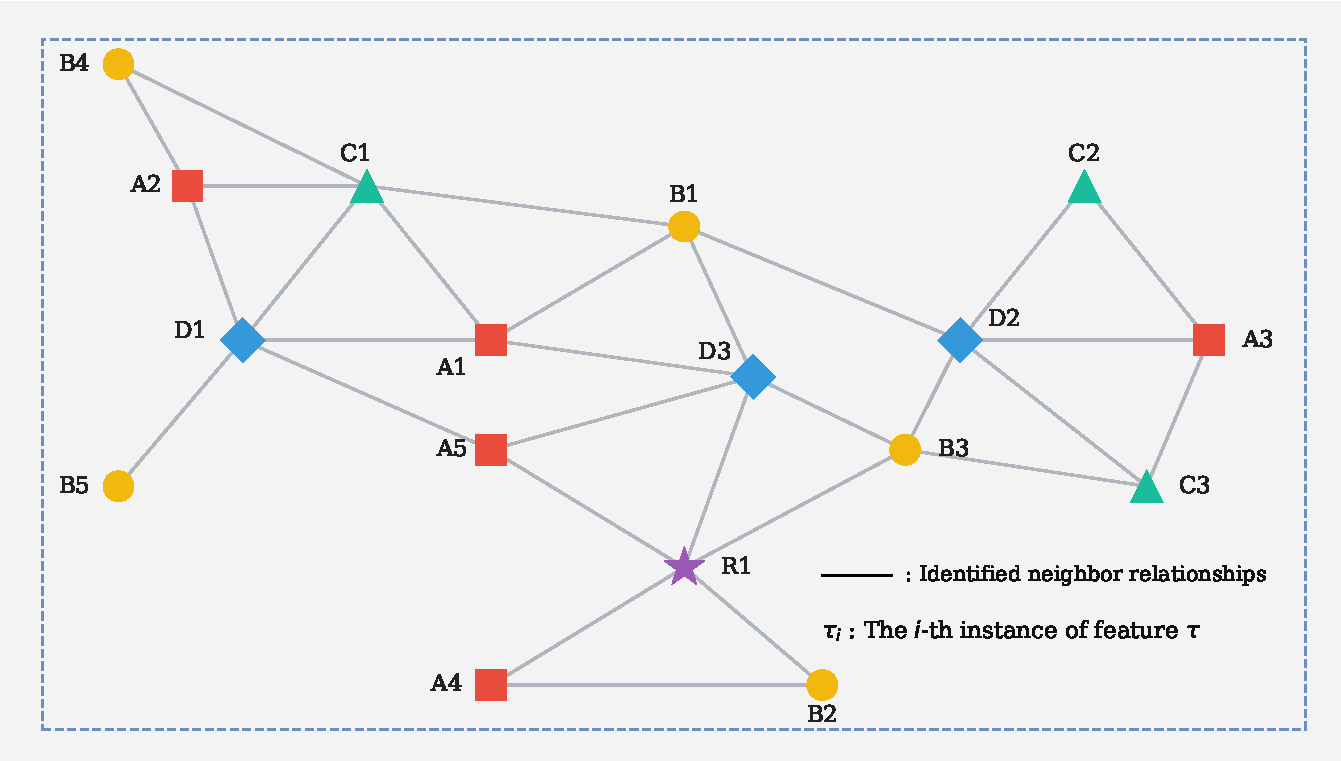
\includegraphics[width=\linewidth]{figures/spatial_network.pdf}
    \caption{Spatial neighborhood graph with rare feature $R$.}
    \label{fig:spatial_network}
\end{figure}

\begin{definition}[Neighborhood and Co-location Instance]
A spatial neighborhood relationship, denoted as $x \sim_{\varepsilon} y$, exists between two objects $x$ and $y$ if their spatial distance satisfies a given threshold $\varepsilon$ (or $d$, e.g., $d = 300\text{m}$) under a specific metric (e.g., Euclidean distance) \cite{huang2004discovering}. Given a candidate SCP, $p \subseteq \mathcal{T}$, ($|p| \ge 2$), a strict type-unique instance of $p$ is defined as a subset of objects $S \subseteq \mathcal{O}$ satisfying two structural constraints: (1) $|S| = |p|$, ensuring a bijective mapping between the objects in $S$ and the feature types in $p$, and (2) all objects in $S$ form a spatial clique (i.e., they are pairwise neighbors) \cite{shekhar2001discovering}. The set of all such instances for pattern $p$ is denoted as $\mathcal{I}(p)$.
\end{definition}

As shown in Figure \ref{fig:spatial_network}, instances satisfying the distance threshold $\varepsilon$ are connected by solid lines. Considering the candidate pattern $p = \{A, D, R\}$, the identified neighbor relationships show that the sole instance $R_{1}$ forms a spatial clique with $A_{5}$ and $D_{3}$. Thus, the co-location instance set is $\mathcal{I}(\{A,D,R\}) = \{\{A_5, D_3, R_1\}\}$.

\begin{definition}[Participation Ratio and Participation Index]
To evaluate the significance of a pattern, we quantify the contribution of each individual feature. The Participation Ratio (PR) of a feature $\tau \in p$ is the fraction of its objects that appear in at least one valid instance of $p$:
\begin{equation}
\text{PR}(\tau \mid p) = \frac{|\mathcal{O}_\tau^p|}{\text{cnt}(\tau)}
\end{equation}
where $\mathcal{O}_\tau^p = \{x \in \mathcal{O}_\tau \mid \exists S \in \mathcal{I}(p), x \in S\}$. Consequently, the Participation Index (PI) of the entire pattern $p$ is bounded by its least participating feature:
\begin{equation}
\text{PI}(p) = \min_{\tau\in p} \{ \text{PR}(\tau \mid p) \}
\end{equation}
A pattern $p$ is deemed a Prevalent Co-location Pattern (PCP) if $\text{PI}(p) \ge \textit{min\_prev}$, where $\textit{min\_prev}$ (or $\mu$) is a user-specified threshold.
\end{definition}

Continuing with the example pattern $p = \{A, D, R\}$, the distinct participating instances for each feature are $\mathcal{O}_A^p = \{A_5\}$, $\mathcal{O}_D^p = \{D_3\}$, and $\mathcal{O}_R^p = \{R_1\}$. Given the total cardinalities $\text{cnt}(A)=5$, $\text{cnt}(D)=3$, and $\text{cnt}(R)=1$, the participation ratios are calculated as $\text{PR}(A \mid p) = \frac{1}{5} = 0.20$, $\text{PR}(D \mid p) = \frac{1}{3} \approx 0.33$, and $\text{PR}(R \mid p) = \frac{1}{1} = 1.00$. Consequently, the overall prevalence degree of this pattern is $\text{PI}(p) = \min \{0.20, 0.33, 1.00\} = 0.20$. If a user sets a minimum prevalence threshold $\textit{min\_prev} = 0.30$, this highly meaningful rare-feature pattern would be prematurely pruned, even though the rare feature $R$ relies entirely on this spatial association.

\subsection{Cauchy Distribution-Based Interest Measure}
\label{sec:cauchy} 

The example in Fig. \ref{fig:spatial_network} is merely a miniature representation of real-world datasets. The actual data contains a massive amount of instances, and the number of instances belonging to each feature varies drastically. To capture such valuable rare-feature co-locations, recent studies introduced the Weighted Participation Index (WPI) \cite{yang2021efficient}, which compensates for feature-frequency disparity by utilizing a Gaussian kernel function to assign relative weights. While conceptually innovative, the exponential nature of the Gaussian weight ($w \propto \exp(v^2)$, where $v$ is the frequency disparity ratio) introduces critical mathematical flaws when applied to massive spatial data \cite{yang2021efficient}. For example, when the illustrative case is scaled to a more realistic setting with $|A| = 1000$ and $|R| = 10$, the frequency disparity becomes $v = 100$. When this value is used in the Gaussian weighting function, the resulting weight can become extremely large, even exceeding $10^{18}$. Such a value may lead to numerical instability and can over-amplify very small participation ratios. Another limitation appears under moderate imbalance. For a pattern such as $p^{\prime} = \{D, R\}$, where $|D| = 30$ and $|R| = 10$ ($v = 3$), the Gaussian weight remains close to $1.0$. As a result, the method provides little adjustment and may still miss moderately rare but meaningful co-location patterns. Consequently, the algorithm offers virtually no compensation, easily leading to the loss of interesting moderately rare patterns. To overcome this mathematical bottleneck, we propose shifting the weighting mechanism to the Lorentzian form of the Cauchy distribution kernel \cite{carrillo2010generalized}.

\begin{definition}[Original Weighted Participation Index \cite{yang2021efficient}]
To compensate for the rare-feature dilemma, the traditional Weighted Participation Index (WPI) evaluates the prevalence of a co-location pattern $p$ by incorporating a rarity-aware weighting mechanism. The metric is defined as:
\begin{equation}
WPI(p) = \min_{\tau \in p} \{PR(\tau \mid p) \cdot weight(\tau, p) \}
\end{equation}
where $weight(\tau, p)$ is the dynamic weight assigned to feature $\tau$, traditionally formulated using a Gaussian kernel function to exponentially amplify the participation ratio of rare features:
\begin{equation}
weight(\tau, p) = \exp\left( \frac{(r(\tau, p) - 1)^2}{2\kappa^2} \right)
\end{equation}
with $r(\tau, p)$ representing the relative frequency disparity of the feature within the pattern, and $\kappa$ serving as the global dispersion parameter of the dataset.
\end{definition}

\begin{definition}[Global Pairwise Dispersion]
Assuming the feature types in $\mathcal{T}$ are indexed in ascending order of their frequencies such that ${cnt}(\tau_1) \le {cnt}(\tau_2) \le \ldots \le {cnt}(\tau_m)$, the global dispersion parameter $\kappa$ is formulated as the arithmetic mean of all pairwise frequency ratios:
\begin{equation}
\label{eq:kappa}
\kappa = \frac{2}{m(m-1)} \sum_{i=1}^{m-1} \sum_{j=i+1}^{m} \frac{{cnt}(\tau_j)}{{cnt}(\tau_i)}
\end{equation}
Functionally, $\kappa$ serves as a global bandwidth parameter that encapsulates the intrinsic frequency skewness across the entire spatial domain.
\end{definition}

\begin{definition}[Cauchy Rare Intensity]
For any candidate pattern $p$, let $\tau_{\min} = \arg\min_{\tau\in p}{cnt}(\tau)$ be its limiting (rarest) feature. We quantify the relative abundance of any feature $\tau \in p$ using the within-pattern ratio $r(\tau,p) = {cnt}(\tau) / {cnt}(\tau_{\min})$. To model the statistical rarity of a feature without aggressive penalization, we define its Rare Intensity (${RI}_{{C}}$) using the Cauchy distribution:
\begin{equation}
RI_C(\tau, p) = \frac{1}{1 + \left(\frac{r(\tau,p)-1}{\kappa}\right)^2}
\end{equation}
\end{definition}

\begin{definition}[Cauchy Distribution-based Weighting]
Unlike the exponential function used in the original WPI (Equation 3), our framework calculates the feature weight $\omega(\tau,p)$ simply as the reciprocal of the Cauchy Rare Intensity:
\begin{equation}
\omega(\tau,p) = \frac{1}{{RI}_{{C}}(\tau, p)} = 1 + \left(\frac{r(\tau,p)-1}{\kappa}\right)^2
\end{equation}
\end{definition}

\vspace{0.5em}
\noindent \textbf{Weight Analysis \& Mathematical Properties:} The polynomial formulation (Equation 5) resolves two main drawbacks of the Gaussian kernel (Equation 4):
\begin{itemize}
\item \textbf{Asymptotic Stability (Preventing Weight Explosion):} Extreme frequency imbalances (large $r$) cause exponential functions to output unmanageable values. Given a global dispersion $\kappa = 8$ and a ratio $r(\tau,p) = 81$, the Gaussian kernel yields $\exp(10^2) \approx 2.68 \times 10^{43}$. This inflation pushes random noise above the prevalence threshold. The Cauchy distribution avoids this via its heavy-tailed polynomial decay \cite{lu2018mining}. Under the same parameters, our Cauchy weight evaluates to $\omega = 1 + 10^2 = 101$. This naturally limits the maximum influence of rare features and prevents false positives.
    
    \item \textbf{Early Sensitivity (Recovering Missed Patterns):} Exponential curves offer minimal compensation for moderate discrepancies (small $r$). Consequently, meaningful spatial patterns with slight imbalances are often pruned. The Cauchy function grows more steadily early on. In our evaluation of a moderately rare pair, the Gaussian model produced a weight of $1.08$, leaving the pattern below the threshold. Our framework assigned a weight of $1.16$. This adjustment is sufficient to retain valid spatial relationships.
\end{itemize}

\begin{definition}[Cauchy Weighted Participation Index]
Replacing the exponential weight with our robust Cauchy weight, we define the Cauchy Weighted Participation Ratio (${WPR}_{{C}}$) by multiplying a feature's raw PR with its dynamically calculated Cauchy weight:
\begin{equation}
{WPR}_{{C}}(\tau \mid p) = {PR}(\tau \mid p) \cdot \omega(\tau,p)
\end{equation}
A spatial co-location pattern is considered prevalent when its Cauchy Weighted Participation Index ($WPI_C$) reaches or exceeds the threshold $min\_prev$. We define $WPI_C(p)$ as the bottleneck $WPR_C$ across all features present in $p$:
\begin{equation}
{WPI}_{{C}}(p) = \min_{\tau\in p}{WPR}_{{C}}(\tau \mid p)
\end{equation}
\end{definition}

\paragraph{Impact of Cauchy Weight on Feature Selection.} 
Equation (6) avoids the instability of exponential scaling. The Cauchy kernel preserves the statistical validity of the prevalence score. In traditional models, inflated weights often eclipse the actual $PR$. Even negligible, coincidental co-occurrences (e.g., ${PR} = 10^{-5}$) are artificially pushed above the $\textit{min\_prev}$ threshold by weights like $10^{43}$, generating severe noise. By replacing the Gaussian kernel with $\omega(\tau, p)$ to ensure a predictable polynomial growth curve while providing early sensitivity, ${WPI}_{{C}}$ guarantees that rare-feature compensation is proportionate across all levels of imbalance. The raw ${PR}$ thus retains its discriminative power: a pattern achieves prevalence only if it exhibits genuine spatial proximity coupled with a mathematically sound weight boost. This optimally filters out frequency-induced noise while recovering moderately rare patterns that the traditional WPI discards.


% =====================================================================
%  MUC 3.3 - THE DESIGNED MCR MINING PIPELINE

\subsection{The Designed MCR Mining Pipeline}
\label{sec:mcr}

Sections~\ref{sec:basic} and~\ref{sec:cauchy} have established, respectively, the formal
definition of a co-location instance and the Cauchy Weighted Participation Index
($WPI_C$) used to judge whether a candidate pattern is prevalent. What remains is the
question of \emph{how} to enumerate candidate patterns and retrieve their participating
instances efficiently. This section answers that question by presenting \textbf{MCR}
(\underline{M}aximal \underline{C}lique-based mining with \underline{R}arity awareness),
the mining pipeline designed in this project.

% ---------------------------------------------------------------------
\subsubsection{Algorithmic Motivation and Pipeline Overview}
\label{subsec:mcr_overview}

\noindent\textbf{Why a level-wise strategy is not applicable.}
Traditional co-location mining algorithms such as the join-based or joinless approaches
follow an Apriori-style, bottom-up traversal: size $k$ patterns are generated only from
prevalent patterns of size $k-1$. This pruning rely entirely on the
\emph{anti-monotone} property of the participation index, which
$PI(p') \ge PI(p)$ whenever $p' \subseteq p$. A pattern that does not satisfy the threshold can
therefore never produce a prevalent superset and its branch may be pruned.

This guarantee does \emph{not} carry over to $WPI_C$. In Section~\ref{sec:cauchy}, the weight of a feature is computed relative to the
\emph{rarest feature of the pattern}, $\tau_{\min}(p) = \arg\min_{\tau \in p} cnt(\tau)$,
through the ratio $r(\tau,p) = cnt(\tau)/cnt(\tau_{\min})$ in the same pattern. Enlarging a
pattern with an even rarer feature shifts $\tau_{\min}$ downwards, inflates every ratio
$r(\tau,\cdot)$, and may increase the weights of the existing features.

\textbf{Loss of anti-monotonicity.} $WPI_C$ is not anti-monotone. A pattern $p$ with $WPI_C(p) < min\_prev$ may have a superset
$p'' \supset p$ with $WPI_C(p'') \ge min\_prev$. This occurs because the inclusion of a rarer feature
in $p''$ raises the weights of all remaining features.

This loss of anti-monotonicity has a direct algorithmic consequence: a bottom-up
generate-and-test framework  rely on $WPI_C$ would be \emph{incomplete}, since it
would prune branches that still contain valid rare-feature patterns. The mining engine must
therefore derive its candidates from a source that does not rely on anti-monotonicity.
Maximal cliques provide exactly such a source.

\noindent\textbf{Pipeline structure.}
MCR decomposes the mining task into four stages, executed once each and in sequence:

\begin{enumerate}
    \item \textbf{Feature statistics.} Count the instances of every feature, sort the
    features by the frequency, and compute the global dispersion $\kappa$
    (Eq.~\ref{eq:kappa}). This stage is performed once and its
    results are reused for every weight computation in next stages.
    \item \textbf{Neighbour graph materialisation.} Convert the raw spatial dataset into an
    undirected graph $G(V,E)$ in which adjacency encodes the $\varepsilon$-neighbourhood
    relation.
    \item \textbf{Maximal clique enumeration and indexing.} Enumerate all maximal cliques of
    $G$ using the MCEHybrid algorithm, then organise them into a \emph{participating
    instance hash table}.
    \item \textbf{Top-down candidate traversal.} Starting from the feature sets of the larger size
    maximal cliques (the largest possible candidates), the algorithm evaluate a candidate with
    $WPI_C$, decides which of its subsets are guaranteed to be prevalent, and push the
    remaining subsets back into a priority queue.
\end{enumerate}

% ---------------------------------------------------------------------
% [HINH 3.x - CAN BO SUNG]
% So do khoi (block diagram) cua toan bo pipeline MCR.
% Goi y noi dung: 5 khoi xep ngang hoac doc:
%   [Spatial dataset O, T]
%      -> (1) Feature statistics  ==> feat_freq, kappa
%      -> (2) Build neighbour graph (epsilon)  ==> G(V,E)
%      -> (3) MCEHybrid + Build hash table     ==> clique_map
%      -> (4) Priority-driven traversal + WPI_C evaluation
%      -> [Output: SCPs]
% Nen ve mui ten phu tu khoi (1) di thang xuong khoi (4) de the hien
% rang feat_freq va kappa duoc dung lai o buoc danh gia.
% Cong cu goi y: draw.io / TikZ. Xuat PDF vector.
% ---------------------------------------------------------------------
\begin{figure}[htbp]
    \centering
    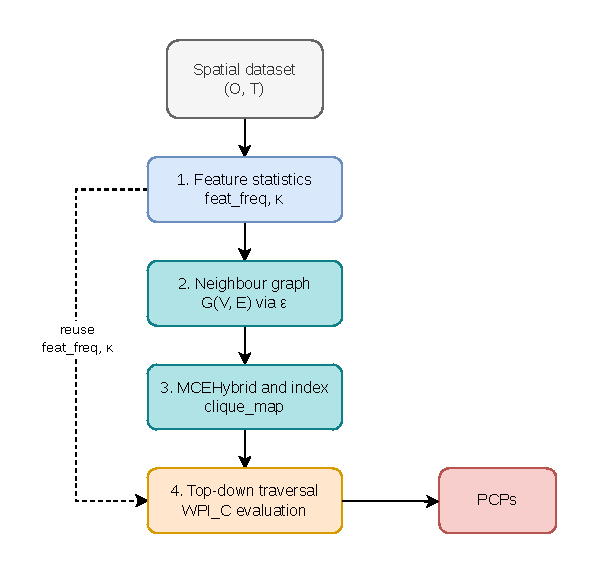
\includegraphics[width=0.9\textwidth]{figures/mcr_pipeline.pdf}
    \caption{Overview of the four-stage MCR mining pipeline.}
    \label{fig:mcr_pipeline}
\end{figure}

Each stage is detailed in the following subsections.

% ---------------------------------------------------------------------
\subsubsection{The MCR Pipeline Stages}
\label{subsec:mcr_pipeline}

\paragraph{Stage 1: Feature Statistics and Rarity Preparation.}
\label{subsec:mcr_feature_stats}
\label{sec:stage1}
\leavevmode\\[0.5em]
Before constructing spatial neighbourhoods, MCR first computes the global statistics required
by the Cauchy weighting mechanism. For each feature type $\tau \in \mathcal{T}$, the number of
instances $cnt(\tau)$ is counted from the input instance set $\mathcal{O}$. The resulting
frequency table is then sorted in ascending order of frequency. Therefore, rare features can be
identified consistently throughout the mining process.

These feature counts serve two purposes. First, they provide the denominators of the
participation ratios $PR(\tau \mid p)$ used when evaluating a candidate pattern. After that, they
are used to compute the global dispersion parameter $\kappa$ defined in
Eq.~\ref{eq:kappa}. Because both $cnt(\tau)$ and $\kappa$ depend only on the input dataset, they
are computed once during the preprocessing step and reused for all subsequent $WPI_C$ evaluations.

This stage is independent of the distance threshold $\varepsilon$ and of the prevalence
threshold $min\_prev$. It therefore separates the rarity-aware weighting preparation from the
spatial neighbourhood construction performed in the next stage.

% ---------------------------------------------------------------------
\paragraph{Stage 2: Neighbour Graph Materialisation.}
\label{subsec:mcr_graph}
\leavevmode\\
After the neighbourhood relationships in Section~\ref{sec:basic} have been
established, the spatial dataset is represented as an undirected graph $G(V,E)$. The vertex
set is the whole instance set, $V \equiv \Psi$, and an edge is created between any two
vertices whose instances satisfy the condition:
\begin{equation}
E = \{\, (x,y) \mid x,y \in \mathcal{O},\; x \neq y,\; dist(\mathbf{s}(x), \mathbf{s}(y)) \le \varepsilon \,\}.
\end{equation}
The graph is unweighted and undirected, since the neighborhood relation
$\sim_{\varepsilon}$ is symmetric and its strength is irrelevant to the clique
condition. Feature labels are not stored on the vertices of $G$ itself.
Instead, a separate mapping $\lambda: V \rightarrow \mathcal{T}$ records the
feature type of each instance. This mapping is consulted only when
constructing the edge set $E$ in Stage~1 to enforce that adjacent
instances belong to different feature types. Once $G$ is built, the cross-feature constraint is already encoded as a structural
invariant of the graph: two instances of the same feature are never adjacent
in $G$. As a result, the clique enumeration algorithms of Stage~2 need not
reference $\lambda$ at all and can operate as purely structural graph
algorithms.

\noindent\textbf{Implementation consideration.}
A naive materialisation compares every pair of instances and therefore costs
$O(n^2)$ distance computations, where $n = |\mathcal{O}|$. Since $\varepsilon$ is typically
small relative to the spatial extent of the dataset, this implementation performs a large number of comparisons and the majority of which are immediately rejected. Our implementation instead
partitions the spatial domain into a uniform grid of cell size $\varepsilon$. Because any two
instances within distance $\varepsilon$ must fall either in the same cell or in one of the
eight surrounding cells, each instance is compared only against the contents of its
$3\times3$ cell neighbourhood. Under a roughly uniform spatial distribution, this reduces the
expected cost to $O(n \cdot \bar{c})$, where $\bar{c}$ is the average number of instances per
cell neighbourhood. The resulting graph is stored as an adjacency list with the size of $O(|E|)$.

% ---------------------------------------------------------------------
\newpage
\paragraph{Stage 3: Maximal Clique Enumeration and Indexing.}
\label{subsec:mcr_mce}

\begin{definition}[Maximal Clique, MC]
\label{def:mc}
A subset of instances $cl = \{o_1, \ldots, o_l\} \subseteq V$ is called a \emph{clique} if
every pair of instances in $cl$ has a neighbouring relationship. A clique $cl$ is a
\emph{maximal clique} if it is not contained in any larger clique $cl'$.
\end{definition}

\noindent\textbf{Why maximal cliques.}
Definition~\ref{def:mc} matches the structural constraint imposed on co-location instances in
Section~\ref{sec:basic}: a valid instance of a pattern is a set of pairwise neighbouring
objects. Every co-location instance is therefore a clique of $G$, and every clique is
contained in at least one maximal clique. This property guarantees that no valid co-location instance is lost when restricting attention to maximal cliques, thereby forming the theoretical basis of the entire pipeline.

\begin{lemma}[Completeness of the clique index]
\label{lem:completeness}
Let $S$ be any co-location
instance of any pattern $p$ with $|p| \ge 2$. Then there exists a maximal
clique $cl$ of $G$ such that $S \subseteq cl$, and consequently
$p \subseteq \lambda(cl)$, where $\lambda(cl) = \{\lambda(o) \mid o \in cl\}$
denotes the feature set of $cl$. Moreover, since edges in $G$ are only
formed between instances of different features, no two instances in $cl$
share the same feature type. Therefore, $\lambda$ restricted to $cl$ is a
bijection, and $|\lambda(cl)| = |cl|$.
\end{lemma}

\begin{proof}
By definition $S$ is a set of pairwise neighbouring instances, hence a clique of $G$. Any
clique of a finite graph can be extended by repeatedly adding adjacent vertices until no
further extension is possible; the resulting set is a maximal clique $cl \supseteq S$.
Applying $\lambda$ to both sides and noting that $S$ contains exactly one instance of each
feature of $p$ gives $p = \lambda(S) \subseteq \lambda(cl)$.
\end{proof}

The completeness of the clique index established above shows that the set
of maximal cliques is a \emph{lossless} summary of the neighbourhood
structure: no participating instance can escape it. This is precisely what allows MCR to abandon the anti-monotone pruning that $WPI_C$ cannot support, as discussed above, without sacrificing
completeness. Since every valid pattern is already guaranteed to appear
within the feature set of some maximal clique, MCR no longer needs
anti-monotone pruning to ensure that no pattern is missed. Candidates are
instead generated directly from maximal cliques during evaluation not as a filter that decides which candidates get generated in the first place.

\noindent\textbf{Scope of this project.}
It should be emphasised that this project does not aim to propose a new maximal clique
enumeration algorithm. The objective is to \emph{exploit} maximal cliques in order to
optimise the co-location pattern mining process. Enumerating all maximal cliques of a graph is an
NP-hard problem, and in the worst case a graph on $n$ vertices may contain $3^{n/3}$ maximal
cliques. Nevertheless, the problem has attracted sustained attention and several algorithms
perform very well on the sparse, locally dense graphs that arise from real spatial data. In
particular, hybrid strategies that adapt the enumeration procedure to the structural
properties of the graph have been shown to improve efficiency in dense neighbourhoods.
This project therefore adopts the \textbf{MCEHybrid} algorithm~\cite{li2019fast}, which
combines the $BK_{rcd}$ and $BK_{pivot}$ variants of the Bron--Kerbosch scheme. Since the
behaviour of this component determines the cost of Stage~2, its mechanics are summarised
below.

\newpage
\noindent\textbf{The Bron--Kerbosch scheme.}
The classical Bron--Kerbosch algorithm~\cite{bron1973algorithm} performs a recursive
backtracking search maintaining three disjoint vertex sets:
\begin{itemize}
    \item $R$ -- the clique currently being built;
    \item $P$ -- the candidate vertices that are adjacent to all vertices of $R$ and may still extend it;
    \item $X$ -- vertices adjacent to all of $R$ that have already been explored, used to avoid reporting duplicates.
\end{itemize}
When both $P$ and $X$ are empty, $R$ cannot be extended by any vertex and is reported as a
maximal clique. Otherwise the algorithm branches on each $v \in P$, recursing on
$R \cup \{v\}$ with $P$ and $X$ restricted to the neighbourhood $N(v)$, and then moves $v$
from $P$ to $X$. The basic scheme is correct but explores many branches that cannot yield a
maximal clique.

\noindent\textbf{Pivoting ($BK_{pivot}$).}
The pivot variant reduces this redundancy. It selects a pivot vertex
$u \in P \cup X$ maximising $|P \cap N(u)|$ and branches only on the vertices of
$P \setminus N(u)$. The justification is that any maximal clique must exclude at least one
of $u$ and its non-neighbours, so branching on the neighbours of $u$ can only reproduce
cliques found elsewhere in the search tree. The branching factor is thereby reduced sharply,
and the effect is strongest when $P$ induces a dense subgraph, since a good pivot then covers
most of $P$.

\noindent\textbf{Degeneracy ordering.}
The outer level of the enumeration is organised around a fixed
\emph{degeneracy ordering} of the vertices, so that each vertex only
searches for cliques among the neighbours that follow it in this order.
For a graph of degeneracy $d$, this bounds the size of every candidate set
by $d$ and yields a worst-case running time of $O(d \cdot n \cdot 3^{d/3})$,
which is near-optimal for globally sparse graphs. Neighbourhood graphs
built from spatial data are typically sparse in this global sense: $d$ is
governed by the local instance density within a radius of $\varepsilon$,
not by $n$, so this bound is far more informative than the generic
$3^{n/3}$ bound. Within each vertex's degeneracy neighbourhood, however,
the induced subgraph is frequently \emph{dense}, and it is this inner
subproblem that the two variants below address.

\noindent\textbf{Recursive core decomposition ($BK_{rcd}$).}
Although pivoting reduces the branching factor, its bottom-up nature adds
only a single vertex to the clique at each level of recursion, which
becomes inefficient in the dense degeneracy neighbourhoods that dominate
real-world graphs. $BK_{rcd}$ addresses this regime with a top-down
strategy: it repeatedly selects and removes the vertex of smallest degree,
applying core decomposition recursively until a clique is reached. It is
therefore substantially more efficient than $BK_{pivot}$ inside dense
degeneracy neighbourhoods.

\noindent\textbf{The hybrid strategy.}
Neither variant dominates the other: $BK_{pivot}$ is effective on the
sparser degeneracy neighbourhoods, where the recursive core decomposition
of $BK_{rcd}$ would only add overhead, whereas $BK_{rcd}$ is markedly
faster inside dense degeneracy neighbourhoods, where the bottom-up
$BK_{pivot}$ stalls. $MCE_{Hybrid}$ therefore evaluates, at each degeneracy
neighbourhood, a cheap structural criterion on the induced subgraph, and
dispatches to $BK_{rcd}$ when the subgraph is dense enough to justify core
decomposition, and to $BK_{pivot}$ otherwise. The precise switching
criterion is given in~\cite{li2019fast}. This is well suited to spatial neighbour graphs, whose defining
characteristic is precisely the coexistence of sparse regions and dense clusters within a
single graph.

% ---------------------------------------------------------------------
% [CHU Y KIEM CHUNG - QUAN TRONG]
% Doan mo ta $BK_{rcd}$ va tieu chi chuyen doi cua MCEHybrid o tren duoc
% viet o muc do khai quat. Ban CAN doc lai [li2019fast] va:
%   (1) Xac nhan chinh xac $BK_{rcd}$ la bien the nao (ten day du, y tuong chinh);
%   (2) Ghi ro tieu chi ma MCEHybrid dung de chuyen giua hai nhanh
%       (nguong mat do? kich thuoc |P|?;
%   (3) Neu bai bao co pseudo-code cua MCEHybrid, nen dua vao day duoi dang
%       Algorithm 3.x kem trich dan nguon - do an duoc phep trinh bay lai
%       thuat toan cua nguoi khac mien la trich dan ro rang.
% Neu khong the xac dinh chinh xac, hay giu nguyen muc khai quat nhu tren
% va them cau: "The precise switching criterion is given in [li2019fast]."
% ---------------------------------------------------------------------

\noindent\textbf{Illustration.}
To demonstrate Definition~3.1, consider the synetic spatial dataset of
Fig.~\ref{fig:spatial_network}. Once the neighbourhood relationships among the
instances have been materialised as described in
Section~\ref{sec:stage1}, the underlying structure is captured by the
neighbour graph. Executing MCEHybrid on this graph extracts the complete
set of maximal cliques listed in Fig.~\ref{fig:fig2a}. Because edges
in $G$ are formed only between instances of different feature types, every
clique of size $\ge 2$ necessarily involves at least two distinct
features. Consequently, the only cliques unable to support a pattern of
size $\ge 2$ are the single-instance cliques, which are discarded before
the next stage.

% ---------------------------------------------------------------------
\paragraph{Participating Instance Hash Table.}
The enumeration of maximal cliques alone is insufficient for the mining
procedure. For an arbitrary candidate pattern $p$, the mining loop must
efficiently determine the set of instances of each feature in $p$ that
participate in at least one co-location instance of $p$. Answering this
query by scanning the entire clique list for every candidate would incur a
high cost. To avoid this, the cliques are indexed by the feature
sets they realise, yielding a structure that supports direct retrieval of
the relevant instances.

\begin{definition}[Participating Instance Hash Table]
\label{def:pih}
Let $V \equiv \mathcal{O}$ be the vertex set of the neighbourhood graph and
let $\lambda(x)$ denote the feature type of an object $x$ (i.e. the unique
$\tau$ with $x \in \mathcal{O}_\tau$). A \emph{participating instance hash
table} is a hash-map whose keys are the feature sets realised by the
maximal cliques. For each key $K$ and each feature $\tau \in K$, the stored
value groups, by feature type, all objects that occur in some maximal
clique whose feature set is exactly $K$:
\begin{equation}
clique\_map[K][\tau] \;=\;
\{\, x \in \mathcal{O} \;\mid\; \exists\, cl \in \mathcal{MC}:\;
\lambda(cl) = K,\; x \in cl,\; \lambda(x) = \tau \,\},
\end{equation}
for every $K \in \{\lambda(cl) \mid cl \in \mathcal{MC}\}$, where
$\mathcal{MC}$ is the set of all maximal cliques and $\lambda(cl)$ the set
of distinct feature types appearing in $cl$.
\end{definition}

Two design decisions deserve comment. First, the key is a \emph{feature
set}, not an object set: this is what makes the index queryable by
pattern, since a pattern is itself a set of features. Second, several
distinct maximal cliques may share the same feature set --- for example
two different geographic locations may each contain one bank, one bus stop
and one hotel. Their objects are therefore merged under the same key,
grouped per feature; consequently each feature group under a key may hold
several objects, even though every individual clique contributes at most
one object per feature (since, by construction, $\lambda$ is a bijection on
each clique).

\noindent\textbf{One instance per feature within a clique.}
Since edges in $G$ are formed only between instances of different feature
types, no maximal clique can contain two instances of the same feature.
Restricted to a clique $cl$, the labelling map $\lambda$ is therefore a
bijection, and $|\lambda(cl)| = |cl|$. Consequently, each clique $cl$
corresponds to exactly one co-location instance of the pattern $\lambda(cl)$, and no per-feature expansion is required when
the clique is queried. Retaining the clique directly is what keeps the
memory footprint low: only the union of participating instances, rather
than a full list of expanded co-location instances, needs to be
materialised in order to compute $PR$.

\noindent\textbf{Query procedure.}
Let $p$ be a candidate pattern. By Lemma~\ref{lem:completeness}, every co-location instance in $\mathcal{I}(p)$ lies
inside some maximal clique whose feature set is a superset of $p$. It is
therefore sufficient to inspect the keys $K \supseteq p$. For each feature
$\tau \in p$, the participating objects $\mathcal{O}_\tau^p$ of
Section~\ref{sec:basic} are recovered directly as the per-feature union
over those keys:
\begin{equation}
\label{eq:query}
\mathcal{O}_\tau^p \;=\;
\bigcup_{\substack{K \in keys(clique\_map) \\ K \supseteq p}}
clique\_map[K][\tau],
\qquad \tau \in p .
\end{equation}
Because the table already groups objects by feature, the query reduces to
a set union within each feature group, with no join \emph{across} feature
groups. The participation ratio then follows immediately as
$PR(\tau \mid p) = |\mathcal{O}_\tau^p| / cnt(\tau)$, from which
$WPR_C(\tau \mid p)$ and $WPI_C(p)$ are obtained as in
Section~\ref{sec:basic}. Crucially, only the per-feature union
$\mathcal{O}_\tau^p$ is materialised; the individual co-location instances
in $\mathcal{I}(p)$ are never enumerated, which is precisely what
eliminates the costly instance join of traditional algorithms.

\noindent\textbf{Example.}
Fig.~\ref{fig:fig2b} illustrates the participating instance hash table generated from all
the maximal cliques of Fig.~\ref{fig:fig2a}. Suppose the candidate pattern
$p = \{A,B\}$ is being evaluated. Following Eq.~\ref{eq:query}, all keys that are supersets of
$\{A,B\}$ are identified, namely $\{A,B,C\}$, $\{A,B,D\}$ and $\{A,B,R\}$. Accessing the
cliques stored under these keys and projecting them onto $\{A,B\}$ yields the valid
co-location instances $\{A_1,B_1\}$, $\{A_2,B_4\}$ and $\{A_1,B_2\}$. Aggregating these
instances returns the complete set of participating instances for the candidate:
$\mathcal{O}_A^{p} = \{A_1, A_2\}$ and $\mathcal{O}_B^{p} = \{B_1, B_2, B_4\}$, from which
$PR(A \mid p) = 2/5 = 0.4$ and $PR(B \mid p) = 3/5 = 0.6$.

\noindent\textbf{Accelerating the superset lookup.}
Evaluating Eq.~\ref{eq:query} by scanning every key of the hash table costs
$O(|keys| \cdot |p|)$ per query. Our implementation avoids this scan by maintaining an
auxiliary inverted index $idx : \mathcal{T} \rightarrow 2^{keys}$ mapping each feature to the
set of keys that contain it. The keys relevant to a candidate $p$ are then obtained as the
intersection $\bigcap_{\tau \in p} idx[\tau]$, which is computed by intersecting the smallest
posting lists first. Because rare features appear in few keys, this heuristic is particularly
effective for exactly the rare-feature patterns this project targets: the shortest posting
list belongs to the rarest feature and immediately bounds the search.

% ---------------------------------------------------------------------
% [HINH 3.x - DUNG LAI HINH DA CO]
% Dung lai Fig 2 cua paper (figs/table_mcs.pdf + figs/hashmap3.pdf).
% Trong do an nen tach thanh HAI hinh rieng, moi hinh mot caption ro rang,
% thay vi gop subfigure (a)/(b) khong co mo ta nhu trong paper:
%   Hinh 3.x: The complete set of maximal cliques extracted from Fig 3.1.
%   Hinh 3.y: The participating instance hash table constructed from Fig 3.x.
% Neu con thoi gian, nen ve them mot hinh nho minh hoa TRUY VAN:
%   to dam 3 key {A,B,C}, {A,B,D}, {A,B,R} va mui ten gom ve tap
%   PartI({A,B}) - se giup nguoi doc hieu Eq. (3.x) ngay lap tuc.
% ---------------------------------------------------------------------
\begin{figure}[htbp]
    \centering
    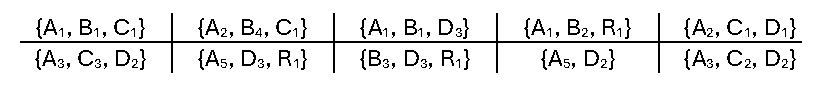
\includegraphics[width=1.0\textwidth]{figures/table_mcs.pdf}
    \caption{The complete set of maximal cliques extracted from the synthetic dataset.}
    \label{fig:fig2a}
\end{figure}

\begin{figure}[htbp]
    \centering
    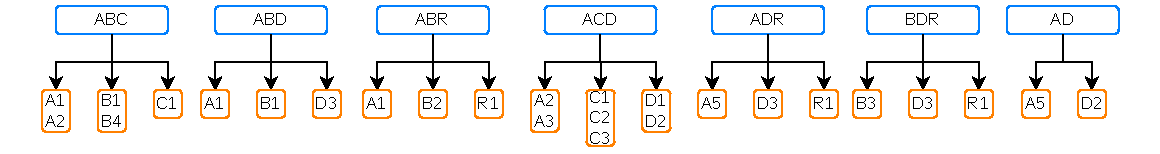
\includegraphics[width=1.0\textwidth]{figures/hashmap3.pdf}
    \caption{The participating instance hash table constructed from the maximal cliques of Fig.~\ref{fig:fig2a}.}
    \label{fig:fig2b}
\end{figure}

% ---------------------------------------------------------------------
\newpage
\paragraph{Stage 4: Top-Down Candidate Traversal.}
\label{subsec:mcr_traversal}
\leavevmode\\[0.5em]
\noindent\textbf{Candidate space and traversal order.}
The keys of the hash table are the starting candidates of the search: by
Lemma~\ref{lem:completeness}, any pattern with at
least one co-location instance in $\mathcal{I}(p)$ is a subset of some key.
Conversely, a pattern that is a subset of no key has
$\mathcal{I}(p) = \emptyset$, hence $PR = 0$ and $WPI_C = 0$. The candidate
space of MCR is therefore exactly the downward closure of the key set, and
the algorithm explores it top-down: the keys form the initial candidates,
and each evaluated candidate spawns its immediate subsets. A max-priority
queue ordered by pattern size drives this traversal, so that larger
patterns are always evaluated before smaller ones. This ordering is not
merely aesthetic --- it is what makes the inference rule of the next
paragraph applicable, since a subset can only be inferred from a superset
that has already been confirmed. A $processed$ set records the patterns
already handled, which is necessary because a pattern of size $k$ can be
reached from several different supersets and would otherwise be evaluated
repeatedly.

\noindent\textbf{Inferring prevalent subsets.}
Although $WPI_C$ is not anti-monotone in general (see the loss of
anti-monotonicity discussed above), a restricted but very useful
monotonicity does hold, and MCR exploits it to skip a large fraction of the
evaluations.

\begin{lemma}[Downward closure under a fixed limiting feature]
\label{lem:inference}
Let $p$ be a pattern with $WPI_C(p) \ge min\_prev$ and let
$\tau_{\min} = \arg\min_{\tau \in p} cnt(\tau)$ be its limiting feature.
Then every subset $q \subseteq p$ with $|q| \ge 2$ and $\tau_{\min} \in q$
satisfies $WPI_C(q) \ge WPI_C(p) \ge min\_prev$, and is therefore prevalent.
\end{lemma}

\begin{proof}
Three observations combine to give the result.

\emph{(i) The weights are unchanged.} Since $q \subseteq p$ and
$\tau_{\min} \in q$, and since $\tau_{\min}$ attains the minimum count over
$p$, it also attains it over $q$; hence $\tau_{\min}$ remains the limiting
feature of $q$ and $cnt(\tau_{\min})$ is unchanged. Because the dispersion
$\kappa$ is a global constant independent of the pattern, for every
$\tau \in q$ the within-pattern ratio is unchanged,
$r(\tau,q) = cnt(\tau)/cnt(\tau_{\min}) = r(\tau,p)$, and consequently
$\omega(\tau,q) = 1 + \big((r(\tau,q)-1)/\kappa\big)^2
= \omega(\tau,p)$.

\emph{(ii) The participation ratios do not decrease.} Let
$S \in \mathcal{I}(p)$. Its projection onto the features of $q$,
$\Pi_q(S) = \{x \in S \mid \lambda(x) \in q\}$, is a set of pairwise
neighbouring objects containing exactly one object per feature of $q$, and
is therefore a co-location instance in $\mathcal{I}(q)$. Hence every object
participating in $p$ also participates in $q$, giving
$\mathcal{O}_\tau^{p} \subseteq \mathcal{O}_\tau^{q}$ and thus
$PR(\tau \mid q) \ge PR(\tau \mid p)$ for all $\tau \in q$.

\emph{(iii) The minimum is taken over fewer terms.} Combining (i) and (ii),
$WPR_C(\tau \mid q) \ge WPR_C(\tau \mid p)$ for every $\tau \in q$. Since
$q \subseteq p$,
\begin{equation*}
\begin{aligned}
WPI_C(q)
&= \min_{\tau \in q} WPR_C(\tau \mid q) \\
&\ge \min_{\tau \in q} WPR_C(\tau \mid p) \\
&\ge \min_{\tau \in p} WPR_C(\tau \mid p)
 = WPI_C(p) \ge min\_prev.
\end{aligned}
\end{equation*}
\end{proof}

Lemma~\ref{lem:inference} is the theoretical basis of the \texttt{InferPrevalentSubsets}
routine. Whenever a candidate $p$ is confirmed prevalent, all of its subsets of size at least
two that retain $\tau_{\min}(p)$ are added to the result set and marked as processed, without
any hash-table query or weight computation. Only the single branch that \emph{drops} the
limiting feature, namely $p \setminus \{\tau_{\min}\}$, has to be pushed back into the queue,
because dropping $\tau_{\min}$ changes the reference point of the weighting function and
invalidates the argument above.

\begin{lemma}[Completeness of the traversal]
\label{lem:traversal_complete}
MCR examines every potentially prevalent pattern; discarding the inferred
subsets from the queue loses no pattern.
\end{lemma}

\begin{proof}
Consider any subset of a confirmed pattern $p$. If it contains
$\tau_{\min}(p)$, it is inferred directly by
Lemma~\ref{lem:inference}. Otherwise it is a subset of
$p \setminus \{\tau_{\min}\}$, which is pushed into the queue and expanded
in turn. Hence no subset of $p$ is lost. Combined with
Lemma~\ref{lem:completeness}, which guarantees that the initial candidate
set covers all patterns with non-empty instance sets, this establishes
that MCR examines every potentially prevalent pattern.
\end{proof}

% ---------------------------------------------------------------------
\subsubsection{The MCR Algorithm}
\label{subsec:mcr_algorithm}

Table~\ref{tab:notation_mcr} summarises the notation used in the pseudo-code, and
Algorithm~\ref{alg:mcr} gives the complete procedure.

\begin{table}[H]
\centering
\caption{Notation used in Algorithm~\ref{alg:mcr}.}
\label{tab:notation_mcr}
\begin{tabularx}{\textwidth}{l X}
\hline
\textbf{Symbol} & \textbf{Meaning} \\
\hline
$\mathcal{O}$, $\mathcal{T}$ & spatial instance set and feature set \\
$\varepsilon$ & distance threshold defining the neighbourhood relation \\
$min\_prev$ & user-specified minimum prevalence threshold \\
$feat\_freq$ & feature-frequency table, sorted in ascending order of count \\
$\kappa$ & global pairwise dispersion of the dataset (Eq.~\ref{eq:kappa}) \\
$G(V,E)$ & neighbour graph over the instances \\
$\mathcal{MC}$ & set of all maximal cliques of $G$ \\
$clique\_map$ & participating instance hash table (Definition~\ref{def:pih}) \\
$PatternQueue$ & max-priority queue of candidate patterns, ordered by size \\
$processed$ & set of patterns already evaluated or inferred \\
$PartI$ & participating objects $\{\mathcal{O}_\tau^p : \tau \in p\}$ of the current candidate (Eq.~\ref{eq:query}) \\
$SCPs$ & output set of rare-feature co-location patterns \\
\hline
\end{tabularx}
\end{table}

\begin{algorithm}[!ht]
\SetAlgoLined
\KwIn{
Spatial instance set $\mathcal{O}$, Feature set $\mathcal{T}$, Distance threshold $\epsilon$, Prevalence threshold $min\_prev$
}
\KwOut{Set of spatial co-location patterns with rare features($SCPs$)}
$feat\_freq \leftarrow \texttt{CountAndSortFeatures}(\mathcal{O}, \mathcal{T})$\;
$\kappa \leftarrow \texttt{CalculateDispersion}(feat\_freq)$\;
$G(V, E) \leftarrow \texttt{BuildNeighborGraph}(\mathcal{O},\epsilon)$\;
$clique\_map \leftarrow \texttt{ExecuteMCEHybrid}(G(V,E))$\;
$PatternQueue \leftarrow \texttt{PriorityQueue}(\texttt{ExtractCandidates}(clique\_map))$\;
$SCPs \leftarrow \emptyset$\;
$processed \leftarrow \emptyset$\;
\While{$PatternQueue$ is not empty}{
    $p \leftarrow PatternQueue.\texttt{pop\_max()}$\;
    \If{$p \in processed$}{
        \textbf{continue}\;
    }
    $processed \leftarrow processed \cup \{p\}$\;
    $PartI \leftarrow \texttt{QueryInstances}(p, clique\_map)$\;
    $RI_c \leftarrow \texttt{CalcRareIntensity}(p, feat\_freq, \kappa)$\;
    $WPI_c \leftarrow \texttt{ComputeWeightedPI}(PartI, p, RI_c, feat\_freq)$\;
    $newCs \leftarrow \texttt{DeriveSubPatterns}(p)$\;
    \If{$WPI_c \geq min\_prev$}{
        $InferredPCPs \leftarrow \texttt{InferPrevalentSubsets}(newCs, p, feat\_freq)$\;
        $SCPs \leftarrow SCPs \cup \{p\} \cup InferredPCPs$\;
        $newCs \leftarrow newCs \setminus InferredPCPs$\;
    }
    \ForEach{$subset \in newCs$}{
        \If{$subset \notin processed$}{
            $PatternQueue.\texttt{push}(subset)$\;
        }
    }
}
\Return $SCPs$\;
\caption{MCR Colocation Mining}
\label{alg:mcr}
\end{algorithm}
\FloatBarrier

\noindent\textbf{Initialisation (lines 1--7).}
The features of the dataset are first counted and sorted, which serves two purposes. The first is to
supply the denominators $cnt(\tau)$ of the participation ratios, and the second allows the global
dispersion $\kappa$ to be computed from the sorted frequency list over the
feature pairs (lines 1--2). The neighbour graph is then constructed from the user-defined
threshold $\varepsilon$ (line 3). MCEHybrid enumerates its maximal cliques and indexes them into the
participating instance hash table (line 4). Finally, the keys of
the hash table are extracted to form the initial candidate set, which is loaded into a
priority queue ordered by pattern size (line 5); the result sets are then initialised as empty
(lines 6--7). Since these preprocessing steps (lines 1--5) depend only on
the input data and not on $min\_prev$, the index they build can be reused across several runs
with different prevalence thresholds, which is a property exploited in the experiments of Section~\ref{chap:experiments}.

\noindent\textbf{Candidate evaluation and generation (lines 8--17).}
The algorithm processes the pattern queue until it is empty. Each iteration extracts the
highest-priority candidate $p$, i.e. the largest unprocessed pattern (line 9). To prevent
redundant computation, it checks whether $p$ has already been handled. If so, it skips to the
next iteration (lines 10--11), otherwise $p$ is recorded as processed (line 13). The participating
instances of $p$ are then retrieved by querying the hash table (line 14). Moreover, the Cauchy rare
intensity of each feature in $p$ is computed from the frequency table and $\kappa$ (line 15).
As a result, the two are combined into the Cauchy weighted participation index $WPI_C(p)$ as defined
in Section~\ref{sec:cauchy} (line 16). Line 17 derives the immediate subsets of $p$, which
constitute the next level of the downward traversal.

\noindent\textbf{Selecting and inferring prevalent co-locations (lines 18--29).}
If $WPI_C(p)$ reaches the minimum prevalence threshold (line 18), $p$ is determined as a
prevalent pattern and added to the output. The algorithm then invokes
\texttt{InferPrevalentSubsets}, which by Lemma~\ref{lem:inference} returns every subset of $p$ that
contains the same rare feature $\tau_{\min}(p)$ (line 19); these are added to the output together
with $p$ itself (line 20). Removing them from $newCs$
(line 21) leaves only the branch that drops the rare feature, which still requires
explicit evaluation. Finally, every remaining unprocessed subset is pushed into the queue for
subsequent processing (lines 23--25). When the queue is exhausted, $SCPs$ contains the
complete set of discovered rare-feature co-location patterns and is returned (line 29).

% ---------------------------------------------------------------------
\subsubsection{An Illustrative Walkthrough}
\label{subsec:mcr_example}

This subsection traces MCR on the synthetic dataset of Fig.~\ref{fig:spatial_network},
whose feature counts are $cnt(A)=5$, $cnt(B)=5$, $cnt(C)=3$, $cnt(D)=3$ and
$cnt(R)=1$, with $\varepsilon$ as drawn and $min\_prev = 0.3$.

\noindent\textbf{Preprocessing.}
Sorting the features by frequency gives the order
$R \prec C \equiv D \prec A \equiv B$. Applying Eq.~\ref{eq:kappa} to the ten
feature pairs yields a global dispersion of $\kappa \approx 2.47$, which
reflects the imbalance introduced by the single instance
of $R$. The neighbour graph is then built and MCEHybrid produces the maximal
cliques of Fig.~\ref{fig:fig2a}, which are indexed into the participating
instance hash table of Fig.~\ref{fig:fig2b} (Definition~\ref{def:pih}). The
keys of the hash table are $\{A,B,C\}$, $\{A,B,D\}$, $\{A,B,R\}$,
$\{A,C,D\}$, $\{A,D,R\}$, $\{B,D,R\}$ and $\{A,D\}$, which become the initial
candidates.

\noindent\textbf{Evaluating a rare-feature candidate.}
Consider the candidate $p = \{A,D,R\}$, which is discarded by the traditional participation index according to Section~\ref{sec:intro}. Its rare feature
is $\tau_{\min} = R$ with $cnt(R) = 1$, so the within-pattern ratios are
$r(R,p) = 1$, $r(D,p) = 3$ and $r(A,p) = 5$. Based on the Cauchy
weighting function of Section~\ref{sec:cauchy} with $\kappa \approx 2.47$, the resulting weights
gives
\[
\omega(R,p) = 1, \qquad
\omega(D,p) = 1 + \left(\tfrac{2}{2.47}\right)^{2} \approx 1.66, \qquad
\omega(A,p) = 1 + \left(\tfrac{4}{2.47}\right)^{2} \approx 3.63 .
\]
Querying the hash table (Eq.~\ref{eq:query}) returns the per-feature
participating objects $\mathcal{O}_A^p = \{A_5\}$,
$\mathcal{O}_D^p = \{D_3\}$ and $\mathcal{O}_R^p = \{R_1\}$. Each feature
contributes a single object, so $p$ is supported by exactly one co-location
instance. Therefore, the participation ratios are $PR(R \mid p) = 1.00$,
$PR(D \mid p) = 1/3 \approx 0.33$ and $PR(A \mid p) = 1/5 = 0.20$, and the
weighted ratios are
\[
WPR_C(R \mid p) = 1.00, \qquad
WPR_C(D \mid p) \approx 0.55, \qquad
WPR_C(A \mid p) \approx 0.73.
\]
From the previous calculation, $WPI_C(p) \approx 0.55$. Since $0.55 \ge min\_prev = 0.30$, the pattern is
confirmed prevalent. For comparison, the unweighted index gives
$PI(p) = \min\{0.20, 0.33, 1.00\} = 0.20$ and would prune this pattern, even
though the rare feature $R$ depends entirely on this spatial association.
This is precisely the recovery behaviour that motivated the Cauchy weighting
framework.

\noindent\textbf{Inference step.}
Because $\tau_{\min}(p) = R$, Lemma~\ref{lem:inference} applies to every
subset of $p$ that retains $R$, namely $\{A,R\}$ and $\{D,R\}$. Both are added
to $SCPs$ and marked as processed without any further computation. Since for $\{D,R\}$ the weights are unchanged and
$WPI_C(\{D,R\}) \approx 0.55 \ge WPI_C(p)$, only the subset $\{A,D\}$, which
drops the rare feature, still requires an independent evaluation. Evaluating it triggers a fresh weighting, since its rare feature
becomes $D$ with $cnt(D) = 3$, the ratios are shrinked to $r(D) = 1$ and
$r(A) = 5/3$, giving $\omega(A) \approx 1.07$ and hence far weaker
compensation. This illustrates concretely why the inference of
Lemma~\ref{lem:inference} cannot be extended to subsets that drop
$\tau_{\min}$.

\noindent\textbf{Full traversal.}
Table~\ref{tab:mcr_walkthrough_trace} traces the complete traversal. First, patterns
are popped from the largest size. For each iteration the table lists the
popped candidate, then calculates $WPI_C$. Whether
it is prevalent, the subsets inferred through Lemma~\ref{lem:inference}, and the subsets pushed onto the
queue. The traversal terminates
after nine iterations and returns $14$ prevalent co-location patterns: the
five size-three patterns $\{A,D,R\}$, $\{A,B,R\}$, $\{B,D,R\}$, $\{A,C,D\}$
and $\{A,B,C\}$, together with nine size-two patterns. The only size-three
candidate rejected is $\{A,B,D\}$, whose $WPI_C = 0.22$ falls below
$min\_prev$. Correspondingly, $\{A,B\}$ and $\{B,D\}$ are still confirmed on
their own once evaluated directly.

\begin{table}[htbp]
\centering
\caption{Iteration trace of the MCR traversal on the synthetic dataset
($min\_prev = 0.3$, $\kappa \approx 2.47$).}
\label{tab:mcr_walkthrough_trace}
\resizebox{\textwidth}{!}{%
\begin{tabular}{clclclll}
\toprule
\textbf{Iter} & \textbf{$p$ popped} & \textbf{$|p|$} &
\textbf{$PartI$ ($\mathcal{O}_\tau^p$ per feature)} & \textbf{$WPI_C$} &
\textbf{Prevalent} & \textbf{Inferred} & \textbf{Pushed} \\
\midrule
1 & $\{A,D,R\}$ & 3 & $A{:}\{A_5\},\ D{:}\{D_3\},\ R{:}\{R_1\}$ & $0.55$ & Yes & $\{A,R\},\{D,R\}$ & --- \\
2 & $\{A,B,R\}$ & 3 & $A{:}\{A_1\},\ B{:}\{B_2\},\ R{:}\{R_1\}$ & $0.73$ & Yes & $\{B,R\}$ & $\{A,B\}$ \\
3 & $\{B,D,R\}$ & 3 & $B{:}\{B_3\},\ D{:}\{D_3\},\ R{:}\{R_1\}$ & $0.55$ & Yes & --- & $\{B,D\}$ \\
4 & $\{A,C,D\}$ & 3 & $A{:}\{A_2,A_3\},\ C{:}\{C_1,C_2,C_3\},\ D{:}\{D_1,D_2\}$ & $0.43$ & Yes & $\{A,C\},\{C,D\}$ & --- \\
5 & $\{A,B,C\}$ & 3 & $A{:}\{A_1,A_2\},\ B{:}\{B_1,B_4\},\ C{:}\{C_1\}$ & $0.33$ & Yes & $\{B,C\}$ & --- \\
6 & $\{A,B,D\}$ & 3 & $A{:}\{A_1\},\ B{:}\{B_1\},\ D{:}\{D_3\}$ & $0.22$ & No & --- & --- \\
7 & $\{A,D\}$ & 2 & $A{:}\{A_1,A_2,A_3,A_5\},\ D{:}\{D_1,D_2,D_3\}$ & $0.86$ & Yes & --- & --- \\
8 & $\{A,B\}$ & 2 & $A{:}\{A_1,A_2\},\ B{:}\{B_1,B_2,B_4\}$ & $0.40$ & Yes & --- & --- \\
9 & $\{B,D\}$ & 2 & $B{:}\{B_1,B_3\},\ D{:}\{D_3\}$ & $0.33$ & Yes & --- & --- \\
\bottomrule
\end{tabular}%
}
\end{table}

% ---------------------------------------------------------------------
\subsubsection{Complexity Analysis}
\label{subsec:mcr_complexity}

Let $n = |\mathcal{O}|$ be the number of instances, $m = |\mathcal{T}|$ the number of
features, $d$ the degeneracy of the neighbour graph, and $M = |\mathcal{MC}|$ the number of
maximal cliques.

\begin{itemize}
    \item \textbf{Feature statistics.} Counting is $O(n)$ and sorting is $O(m \log m)$. The
    dispersion $\kappa$ requires $O(m^2)$ pair evaluations. Since $m \ll n$ in every dataset
    considered in this project, this stage is negligible.

    \item \textbf{Neighbour graph.} $O(n^2)$ in the naive implementation, reduced to
    $O(n \cdot \bar{c})$ on average by the grid partitioning of
    Section~\ref{subsec:mcr_graph}. Storage is $O(n + |E|)$.

    \item \textbf{Maximal clique enumeration.} In the worst case , it costs $O(d \cdot n \cdot 3^{d/3})$ for the
    ordering-based branch. The decisive observation is that $d$ depends on the local instance
    density within radius $\varepsilon$ rather than on $n$, so enlarging the dataset over a
    proportionally larger area increases the cost linearly. This is the structural
    reason for the scalability reported in Section~\ref{sec:scalability}.

    \item \textbf{Hash table construction.} A single pass over the cliques, $O(\sum_{cl \in \mathcal{MC}} |cl|)$
    time and $O(M)$ entries of storage. No co-location instance is materialised at this point.

    \item \textbf{Candidate traversal.} Each query costs $O(|\mathcal{K}_p| \cdot \bar{s})$,
    where $\mathcal{K}_p$ is the set of keys containing $p$ and $\bar{s}$ the average clique size. The number of evaluations is bounded by the
    size of the downward closure of the key set, and is reduced further by
    Lemma~\ref{lem:inference}, which removes from evaluation all subsets retaining the
    limiting feature. Since keys are bounded by $m$ features, this closure is far smaller than
    the $2^m$ theoretical boundz in practice.
\end{itemize}

\noindent\textbf{Comparison with existing paradigms.}
The join-based and joinless algorithms materialise the pattern level by level, using a table of row instances
for every candidate. Therefore, their memory grows with the number of co-location instances, which
explodes as $\varepsilon$ increases. The NR-tree used by the original WPI method removes many
redundant joins but still pays for constructing and traversing an ordered neighbourhood
index. MCR replaces both with a single hash lookup over a structure built once. Participating
instances are retrieved by key intersection rather than by joining, and the expansion of
cliques into instances is performed lazily. This explains the reduced and \emph{stable} memory footprint observed experimentally in
Section~\ref{sec:efficiency}, even when the search space expands significantly.

% ---------------------------------------------------------------------
% [CHU Y CHEO]
% Cac \ref sau day tro toi cac muc khac trong do an - hay doi lai cho khop
% voi nhan (label) thuc te ma ban dat:
%   \ref{sec:basic}         -> muc 3.1
%   \ref{sec:cauchy}        -> muc 3.2
%   \ref{eq:kappa}          -> cong thuc dinh nghia kappa trong muc 3.2
%   \ref{sec:intro}         -> chuong 1
%   \ref{chap:experiments}  -> chuong 5
%   \ref{sec:efficiency}    -> muc 5.3
%   \ref{sec:scalability}   -> muc 5.4
%   \ref{fig:intro -> hinh synthetic dataset trong muc 3.1
% ---------------------------------------------------------------------
\section{Dataset} \label{dataset}

The experimental evaluation uses two groups of datasets corresponding to two
different tasks in this thesis. The first group consists of four real-world
spatial POI datasets, namely Las Vegas, Toronto, Shanghai, and Beijing, which are
used to evaluate spatial co-location pattern mining. In these datasets, each
record represents a spatial instance associated with a feature type and a
two-dimensional location. The second group consists of two city-scale Yelp POI
datasets, Philadelphia and New Orleans, used for the downstream task; each record
is a venue with a category label, geographic coordinates, and a user star rating.
Since these two groups serve different experimental purposes, they are reported
separately in the following subsections.

\subsection{Dataset Overview and Imbalance Statistics}\label{class-wise}

\vspace{4pt}
\noindent\textbf{Datasets for Spatial Co-location Pattern Mining}
\vspace{2pt}

The proposed method is evaluated on four real-world datasets, namely Las Vegas,
Toronto, Shanghai, and Beijing. The Las Vegas dataset is extracted from the Yelp
Open Dataset\footnote{\url{https://business.yelp.com/data/resources/open-dataset}},
covering a range of venue categories in the United States. The remaining three
datasets are constructed from public Point-of-Interest (POI)
sources~\cite{tran2023efficient,bao2019clique,tran2021mcht} and undergo a
preprocessing stage to eliminate invalid records.

\begin{table}[h]
\centering
\caption{Characteristics of the four real-world datasets.}
\label{tab:dataset}
\begin{tabular}{lcccc}
\toprule
\textbf{Dataset} & \textbf{\ Features} & \textbf{\ Instances} & \textbf{Spatial Coverage} & \textbf{$\kappa$} \\
\midrule
Las Vegas & 17 & 22{,}725 & $38{,}649 \times 62{,}985$~km$^2$ & 2.90 \\
Toronto   & 20 & 17{,}129 & $23{,}417 \times 56{,}036$~km$^2$ & 7.86 \\
Shanghai  & 14 & 41{,}454 & $65{,}557 \times 113{,}690$~km$^2$ & 13.22 \\
Beijing   & 19 & 104{,}909 & $138.7 \times 227$~km$^2$ & 16.74 \\
\bottomrule
\end{tabular}
\end{table}

Table~\ref{tab:dataset} summarises the key characteristics of each dataset.
Beyond the basic statistics --- the number of feature types, the total number of
instances, and the spatial coverage --- the table reports the global dispersion
$\kappa$ defined in the Methodology. This quantity captures the difference in
instance counts across all feature pairs: a higher $\kappa$ indicates a larger
imbalance in feature frequencies and therefore more pronounced rare-feature
characteristics, whereas a lower $\kappa$ implies a relatively uniform
distribution. The four datasets deliberately span a wide range of $\kappa$
(from 2.90 for Las Vegas up to 16.74 for Beijing), which provides a comprehensive
basis for assessing the behaviour of rare-feature discovery strategies under
varying degrees of skewness. Unless otherwise stated, all experiments use these
$\kappa$ values as the global dispersion parameter of the weighting functions.

\begin{table}[h]
\centering
\caption{Feature-frequency imbalance statistics of the SCP mining datasets.}
\label{tab:imbalance_stats}
\begin{tabular}{lrrrr}
\toprule
\textbf{Dataset} 
& \textbf{Min Count} 
& \textbf{Median Count} 
& \textbf{Max Count} 
& \textbf{IR} \\
\midrule
Las Vegas & 304 & 924.0   & 4{,}534  & 14.91 \\
Toronto   & 270 & 497.5   & 5{,}304  & 19.64 \\
Shanghai  & 112 & 909.5   & 9{,}110  & 81.34 \\
Beijing   & 75  & 3{,}493.0 & 22{,}530 & 300.40 \\
\bottomrule
\end{tabular}
\end{table}

Table~\ref{tab:imbalance_stats} reports additional feature-frequency imbalance
statistics for the four SCP mining datasets. Let $cnt(\tau)$ denote the number
of instances of feature type $\tau$. The imbalance ratio is defined as
\[
IR = \frac{\max_{\tau} cnt(\tau)}{\min_{\tau} cnt(\tau)}.
\]
While the minimum, median, and maximum counts provide a direct summary of the
feature-frequency range, IR captures the extreme disparity between the most
frequent and the rarest feature types, where a larger value indicates a more
skewed and long-tailed distribution.

The results show that the four datasets exhibit different levels of imbalance.
Las Vegas has the mildest feature-frequency skewness, with an IR of 14.91. In
contrast, Beijing shows the most extreme frequency disparity, where the most
frequent feature contains 22{,}530 instances while the rarest feature contains
only 75 instances, resulting in an IR of 300.40. These statistics confirm that
the selected datasets cover a wide range of imbalance levels, making them
suitable for evaluating rare-feature-aware spatial co-location mining.

\vspace{6pt}
\noindent\textbf{Downstream POI Datasets}
\vspace{2pt}

Two city-scale datasets, Philadelphia and New Orleans, are used for the
downstream task. Unlike the SCP mining datasets, their coordinates are geographic
(latitude/longitude) and have been projected onto a local kilometre plane for
visualisation, and their feature types correspond to real-world POI categories.
The mapping between the feature-map codes used in the figures and their category
names is given in Table~\ref{tab:philly_feature_map} for Philadelphia.

\begin{table}[H]
\centering
\caption{Mapping between feature-map codes and POI categories in the
Philadelphia dataset.}
\label{tab:philly_feature_map}
\begin{tabular}{cl|cl}
\toprule
\textbf{Feature} & \textbf{Category} & \textbf{Feature} & \textbf{Category} \\
\midrule
A & Restaurants        & K & Automotive \\
B & Food               & L & Coffee \& Tea \\
C & Shopping           & M & Sandwiches \\
D & Beauty \& Spas     & N & Pizza \\
E & Home Services      & O & Active Life \\
F & Health \& Medical  & P & Arts \& Entertainment \\
G & Nightlife          & Q & American (Traditional) \\
H & Local Services     & R & Hair Salons \\
I & Bars               & S & Breakfast \& Brunch \\
J & Event Planning \& Services & T & American (New) \\
\bottomrule
\end{tabular}
\end{table}

\begin{table}[H]
\centering
\caption{Overview and rating statistics of the two downstream POI datasets.}
\label{tab:downstream_overview}
\begin{tabular}{lrr}
\toprule
\textbf{Property} & \textbf{Philadelphia} & \textbf{New Orleans} \\
\midrule
\# Feature (categories)     & 20              & 19              \\
\# Instances (POIs)         & 9{,}928         & 2{,}425         \\
Min / Median / Max count    & 91 / 330.5 / 1{,}933 & 63 / 133.0 / 174 \\
Imbalance ratio (IR)        & 21.24           & 2.76            \\
\midrule
Star rating range           & 1.0 -- 5.0      & 1.0 -- 5.0      \\
Overall average rating      & 3.66            & 3.82            \\
Per-category average range  & 3.28 -- 4.17    & 2.43 -- 4.32    \\
\bottomrule
\end{tabular}
\end{table}

Table~\ref{tab:downstream_overview} summarises the two datasets. Philadelphia is
the larger and more skewed of the two, with 9{,}928 POIs across 20 categories and
a moderate feature-frequency imbalance (IR $= 21.24$), whereas New Orleans is
smaller and far more balanced, with 2{,}425 POIs across 19 categories (IR $=
2.76$). In both cases each POI carries a user star rating on a $1$--$5$ scale,
with overall averages of $3.66$ and $3.82$ respectively; the per-category
averages remain within a limited band and do not track category frequency,
indicating that rating quality is largely independent of how frequent a category
is.

\subsection{Spatial Distribution and Visualization} 

\vspace{4pt}
\noindent\textbf{Spatial Distribution of SCP Mining Datasets}
\vspace{2pt}

Rather than visualising all four datasets, we focus on the two lying at the
extremes of the global dispersion range: Las Vegas ($\kappa = 2.90$), the most
balanced, and Beijing ($\kappa = 16.74$), the most skewed. These two bracket the
behaviour of the remaining datasets across three complementary views.

\paragraph{Spatial scatter.}

\begin{figure}[htbp]
    \centering
    \begin{subfigure}[b]{0.4\textwidth}
        \centering
        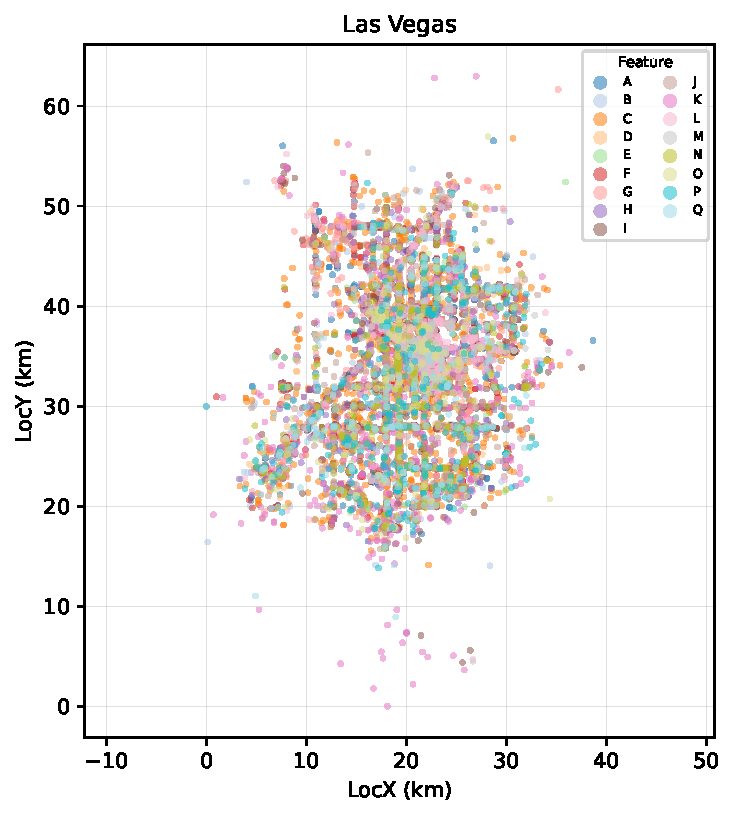
\includegraphics[width=\textwidth]{figures/scatter_sample_lasvegas.pdf}
        \caption{Las Vegas}
        \label{fig:scatter_lasvegas}
    \end{subfigure}
    \hfill
    \begin{subfigure}[b]{0.4\textwidth}
        \centering
        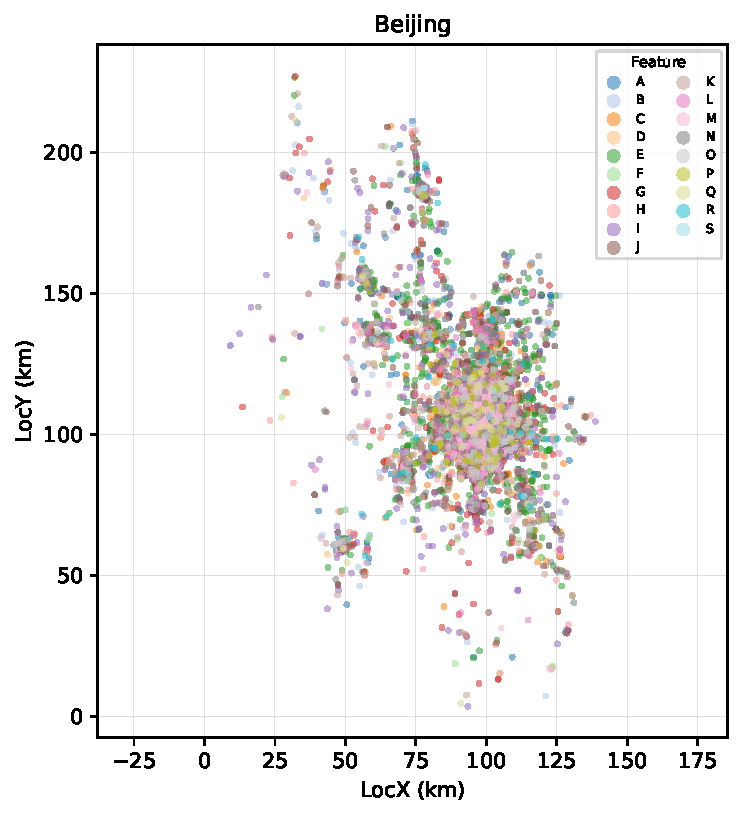
\includegraphics[width=\textwidth]{figures/scatter_sample_beijing.pdf}
        \caption{Beijing}
        \label{fig:scatter_beijing}
    \end{subfigure}
    \caption{Spatial distribution of instances in the Las Vegas and Beijing
    datasets.}
    \label{fig:scatter_distribution}
\end{figure}

Figure~\ref{fig:scatter_distribution} shows the spatial distribution of
instances, with each colour denoting a feature type. Beijing spans a
considerably larger area and contains several times more instances than Las
Vegas, yet in both datasets the instances are spatially non-uniform, forming
tightly packed concentrations alongside sparsely populated regions. Crucially,
different feature types are spatially interleaved rather than segregated, which
is the necessary precondition for co-location patterns to arise.

\paragraph{Density map.}

\begin{figure}[H]
    \centering
    \begin{subfigure}[b]{0.4\textwidth}
        \centering
        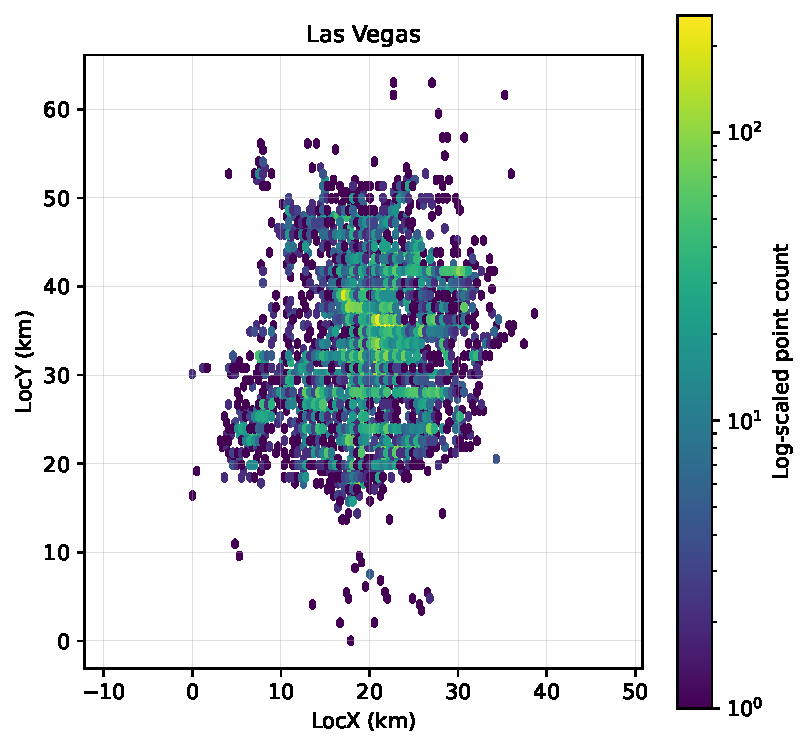
\includegraphics[width=\textwidth]{figures/hexbin_density_lasvegas.pdf}
        \caption{Las Vegas}
        \label{fig:hexbin_lasvegas}
    \end{subfigure}
    \hfill
    \begin{subfigure}[b]{0.4\textwidth}
        \centering
        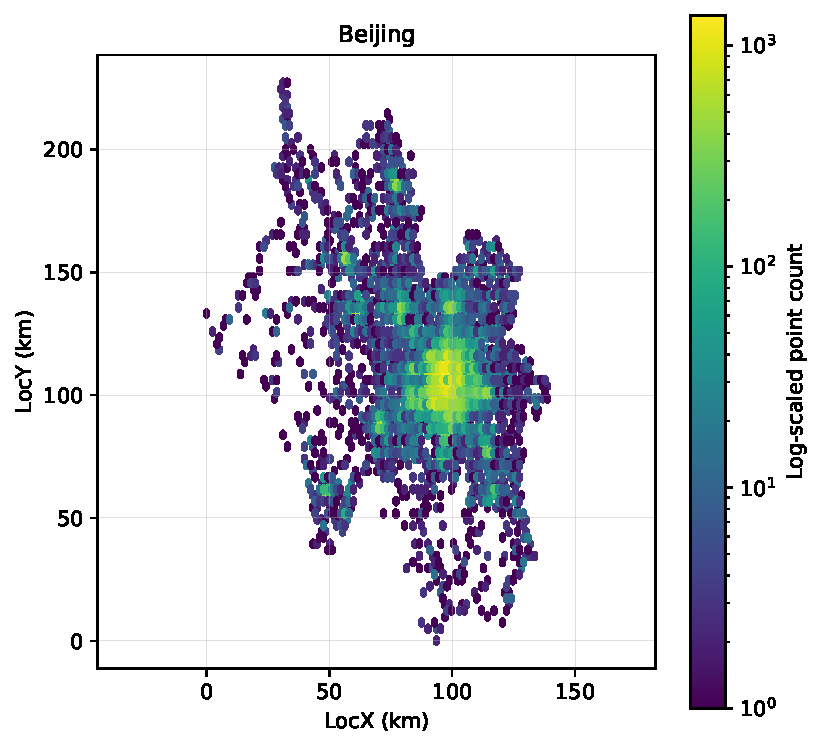
\includegraphics[width=\textwidth]{figures/hexbin_density_beijing.pdf}
        \caption{Beijing}
        \label{fig:hexbin_beijing}
    \end{subfigure}
    \caption{Hexbin density maps of instance distribution in the Las Vegas and
    Beijing datasets.}
    \label{fig:hexbin_density}
\end{figure}

The hexbin maps in Fig.~\ref{fig:hexbin_density} aggregate instances into
hexagonal cells coloured by log-scaled count, exposing the full range of local
densities that the scatter plots saturate. In both datasets a few cells
concentrate a disproportionate share of instances as bright density peaks, while
surrounding regions stay sparse; the contrast is stronger in Beijing, with
several distinct high-density cores. This uneven density directly governs clique
size during mining - dense cells yield large, tightly connected cliques and
sparse cells only small ones---which is what makes an adaptive enumeration
strategy preferable to a fixed one.

\paragraph{Feature-frequency long tail.}

\begin{figure}[H]
    \centering
    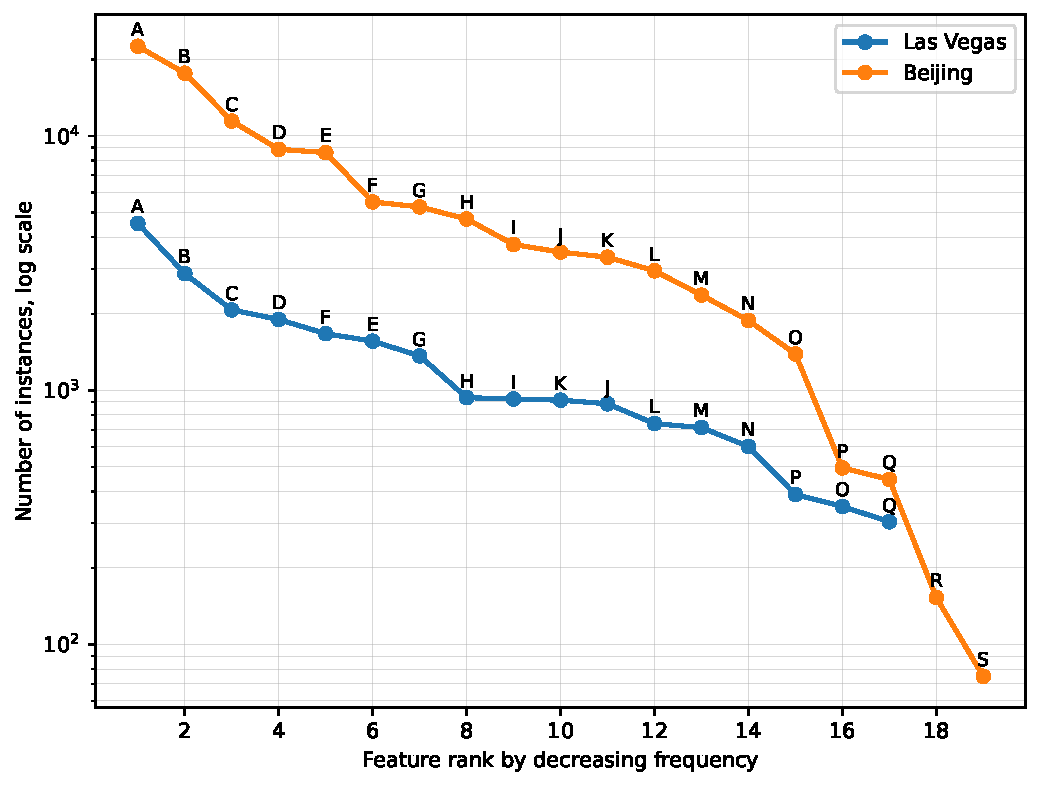
\includegraphics[width=0.85\textwidth]{figures/fig_feature_long_tail_lasvegas_beijing.pdf}
    \caption{Feature-frequency long-tail distributions of the Las Vegas and Beijing datasets.}
    \label{fig:long_tail}
\end{figure}

Figure~\ref{fig:long_tail} ranks each feature by its instance count, translating
the dispersion statistics of Table~\ref{tab:imbalance_stats} into visual form.
The Las Vegas curve descends gently, keeping even its rarest feature within one
order of magnitude of its most frequent one, whereas the Beijing curve falls
steeply into a long, flat tail spanning more than two orders of magnitude on the
logarithmic axis. This illustrates why a bottleneck measure such as the plain
participation index is inadequate: the rare features in the tail carry the most
spatial significance yet are the first to be suppressed under imbalance---exactly
the regime the proposed weighting scheme is designed to accommodate.

\vspace{6pt}
\noindent\textbf{Spatial Distribution of the Downstream Datasets}
\vspace{2pt}

For both Philadelphia and New Orleans, the POIs concentrate in a compact central
urban core and thin out towards the periphery, with a few isolated outliers.
Different categories are spatially interleaved throughout the built-up area
rather than segregated, indicating rich local co-occurrence among POI types---the
setting in which co-location signals are expected to be most informative for the
downstream task. Consistent with Table~\ref{tab:downstream_overview}, the two
datasets differ mainly in scale and skewness: Philadelphia forms a larger and
more strongly concentrated core dominated by \emph{Restaurants}, whereas New
Orleans is smaller and more evenly balanced across categories.


% =====================================================================
%  SECTION 5 - EXPERIMENTS AND ANALYSIS
%  Graft target: thesis using \documentclass[12pt]{template}
%  Requires packages already loaded in the thesis preamble:
%     natbib, amsmath, algorithm2e, booktabs, multirow, subfig,
%     graphicx, makecell, xcolor, placeins
%  \minprev is defined in the preamble as \newcommand{\minprev}{\mathit{minprev}}
%
%  Bibliography keys used here (make sure they exist in the thesis .bib):
%     joinless2006      -> Yoo & Shekhar, joinless PI
%     huang2006mining   -> Huang et al., MaxPR
%     yang2021efficient -> Yang et al., WPI + NR-tree
%     li2019fast        -> Li et al., MCEHybrid
%     tran2023efficient, bao2019clique, tran2021mcht -> POI dataset sources
%
%  Figure paths reuse the paper's exported PDFs under visualization_result/.
%  Cross-reference labels sec:efficiency and sec:scalability are DEFINED here
%  so the forward references in the Methodology (MCR) section resolve.
% =====================================================================

% ---------------------------------------------------------------------
\section{Experiments and Analysis}
\label{chap:experiments}

This chapter evaluates the proposed approach at three levels. First, the
pattern-level experiment examines how Cauchy weighting affects prevalence
decisions under feature-frequency imbalance. Second, the system-level
experiments compare runtime, peak memory, and scalability.

% ---------------------------------------------------------------------
\subsection{Experimental Setup and Baseline Comparison}
\label{sec:exp_setup}

Four mining methods are evaluated. \textbf{PI}~\cite{yoo2006joinless} is the
classical participation-index baseline. \textbf{MaxPR}~\cite{huang2006mining}
uses the maximum participation ratio to identify patterns containing rare
features. \textbf{WPI}~\cite{yang2021efficient} combines Gaussian rarity
weighting with an Ordered NR-tree. \textbf{Ours (MCR)} combines the proposed
Cauchy Weighted Participation Index, $WPI_C$, with MCEHybrid and the hash-based
participating-instance organization described in Section~\ref{sec:mcr}. For
each comparison, the methods were executed with the same input data and
parameter settings.

The experiments were conducted on an
Intel\textsuperscript{\textregistered} Core\texttrademark{} i7-12700H CPU
with 16~GB of RAM and Windows~11. Each method--configuration pair was executed
four times. Runtime includes data loading and pattern mining, while memory is
measured as the peak process working set. All reported runtime and memory
values are arithmetic means over the four runs.

Dataset characteristics and feature-imbalance statistics are presented in
Section~\ref{class-wise}. Table~\ref{tab:exp_parameters} summarizes the
parameters used in the experiments. During each parameter sweep, the parameter
not being varied was fixed at its default value.

\begin{table}[H]
\centering
\small
\caption{Parameter settings used in the mining experiments.}
\label{tab:exp_parameters}
\resizebox{\textwidth}{!}{%
\begin{tabular}{lcccc}
\toprule
\textbf{Dataset} &
\textbf{Default $\varepsilon$} &
\textbf{Default $\minprev$} &
\textbf{Distance sweep} &
\textbf{Prevalence sweep} \\
\midrule
Las Vegas
& 160~m
& 0.15
& 40--200~m, step 40~m
& 0.10--0.30, step 0.05 \\

Toronto
& 120~m
& 0.20
& 100--140~m, step 10~m
& 0.10--0.30, step 0.05 \\

Shanghai
& 250~m
& 0.20
& 150--350~m, step 50~m
& 0.10--0.30, step 0.05 \\

Beijing
& 250~m
& 0.20
& 100--300~m, step 50~m
& 0.10--0.30, step 0.05 \\
\bottomrule
\end{tabular}%
}
\end{table}

% ---------------------------------------------------------------------
\subsection{Effectiveness in Pattern Discovery}
\label{sec:effectiveness}

The imbalance statistics in Table~\ref{tab:imbalance_stats} and the long-tail
distributions in Figure~\ref{fig:long_tail} show substantial differences in
feature frequencies. Since PI is defined by the minimum participation ratio,
an abundant feature may become the bottleneck when it forms a pattern with a
much rarer feature. Consequently, a pattern can receive a low PI even when a
large proportion of the rare-feature instances participate in the spatial
association.

Both Gaussian-WPI and Cauchy-WPI compensate for this imbalance, but their
weight-growth rates lead to different prevalence decisions. Under moderate
frequency disparity, the Cauchy form provides stronger compensation than the
Gaussian form. Under severe disparity, its polynomial growth remains much
smaller than the exponential Gaussian weight. Cauchy-WPI is therefore designed
to improve sensitivity to moderately imbalanced patterns while limiting the
influence of extreme frequency ratios.

The Toronto case study uses $\varepsilon=120$~m and $\minprev=0.2$.
Table~\ref{tab:pattern_comparison} presents four patterns for which the two
weighting functions produce different decisions.

\begin{table}[tbp]
\centering
\caption{Toronto patterns with different Gaussian-WPI and Cauchy-WPI
decisions ($\varepsilon=120$~m and $\minprev=0.2$).}
\label{tab:pattern_comparison}
\resizebox{\textwidth}{!}{%
\begin{tabular}{|c|l|cc|cc|}
\hline
\multirow{2}{*}{\textbf{Acceptance group}}
  & \multirow{2}{*}{\textbf{Pattern}}
  & \multicolumn{2}{c|}{\textbf{Gaussian-WPI}}
  & \multicolumn{2}{c|}{\textbf{Cauchy-WPI}} \\
\cline{3-6}
  & & \textbf{WPRs} & \textbf{Weights}
    & \textbf{WPRs} & \textbf{Weights} \\
\hline
\multirow{2}{*}{\makecell{\textbf{Cauchy-WPI}\\\textbf{only}}}
  & $\{R,E\}$
    & $[0.4661,\ 0.1894]$
    & $[1.0,\ 2.08]$
    & $[0.4661,\ \mathbf{0.2245}]$
    & $[1.0,\ \mathbf{2.46}]$ \\
\cline{2-6}
  & $\{S,F\}$
    & $[0.6000,\ 0.1902]$
    & $[1.0,\ 1.46]$
    & $[0.6000,\ \mathbf{0.2289}]$
    & $[1.0,\ \mathbf{1.76}]$ \\
\hline
\multirow{2}{*}{\makecell{\textbf{Gaussian-WPI}\\\textbf{only}}}
  & $\{T,G,C\}$
    & $[0.2857,\ 0.5986,\ 4.60{\times}10^{10}]$
    & $[1.0,\ 27.35,\ \mathbf{7.19{\times}10^{12}}]$
    & $[0.2857,\ 0.1667,\ 0.3848]$
    & $[1.0,\ 7.62,\ \mathbf{60.21}]$ \\
\cline{2-6}
  & $\{T,G,D\}$
    & $[0.2500,\ 0.6447,\ 2.10{\times}10^{6}]$
    & $[1.0,\ 27.35,\ \mathbf{1.82{\times}10^{8}}]$
    & $[0.2500,\ 0.1795,\ 0.4510]$
    & $[1.0,\ 7.62,\ \mathbf{39.04}]$ \\
\hline
\end{tabular}%
}
\end{table}

For $\{R,E\}$ and $\{S,F\}$, Cauchy weighting raises the bottleneck WPRs
from 0.1894 and 0.1902 to 0.2245 and 0.2289, respectively. Both patterns
therefore cross the prevalence threshold. These examples illustrate the
stronger adjustment provided by the Cauchy form under moderate frequency
imbalance.

For $\{T,G,C\}$ and $\{T,G,D\}$, Gaussian-WPI assigns weights of
$7.19{\times}10^{12}$ and $1.82{\times}10^{8}$. These weights cause the
patterns to exceed the threshold despite their small underlying participation
ratios. Cauchy-WPI limits the corresponding weights to 60.21 and 39.04,
resulting in bottleneck WPRs of 0.1667 and 0.1795. The patterns therefore
remain below the threshold. This behavior shows how polynomial weighting
reduces the effect of extreme frequency ratios on the final decision.

\begin{table}[tbp]
\centering
\small
\caption{Overlap between the Gaussian-WPI and Cauchy-WPI acceptance sets
on Toronto.}
\label{tab:pattern_counts}
\begin{tabular}{ccccc}
\toprule
\textbf{Gaussian-WPI} &
\textbf{Cauchy-WPI} &
\textbf{Both} &
\textbf{Cauchy only} &
\textbf{Gaussian only} \\
\midrule
616 & 647 & 581 & 66 & 35 \\
\bottomrule
\end{tabular}
\end{table}

Gaussian-WPI accepts 616 patterns, whereas Cauchy-WPI accepts 647. The two
methods agree on 581 patterns but make different decisions for 101 patterns.
Cauchy-WPI uniquely accepts 66 patterns, compared with 35 patterns accepted
only by Gaussian-WPI.

The higher Cauchy acceptance count does not result from uniformly increasing
all prevalence scores. Instead, the method accepts additional patterns under
moderate imbalance while keeping patterns dominated by extreme Gaussian
weights below the threshold. The case study therefore supports the intended
advantage of Cauchy weighting: stronger compensation in the moderate regime
and more controlled amplification in the extreme regime. This experiment
evaluates numerical behavior and threshold decisions; validating the semantic
meaning of individual patterns would require external domain annotations.

\FloatBarrier

% ---------------------------------------------------------------------
\subsection{Computational Efficiency: Time and Memory}
\label{sec:efficiency}

The parameter-sensitivity experiments cover Las Vegas, Toronto, and Shanghai.
For each dataset, five distance thresholds and five prevalence thresholds are
evaluated, giving 30 method--configuration comparisons. The proposed MCR
method, denoted as Ours in the figures, records the lowest mean runtime in
25 of the 30 configurations and the lowest mean peak memory in 27
configurations.

The five runtime exceptions occur in relatively sparse or strongly pruned
workloads, where the simpler baselines have lower fixed overhead. At
$\varepsilon=120$~m on Las Vegas, MaxPR requires 6.668~s, compared with
7.038~s for Ours. PI is also faster at $\minprev=0.20$, 0.25, and 0.30 on
Las Vegas, while MaxPR is faster at $\minprev=0.30$ on Toronto
(13.423~s versus 14.530~s). These exceptions indicate that the additional
organization performed by MCR is not always beneficial when the evaluated
search space is small.

The three memory exceptions occur at $\varepsilon=40$~m and 80~m on Las
Vegas and at $\varepsilon=150$~m on Shanghai. In the remaining 27
configurations, Ours records the lowest mean peak memory. Its memory advantage
becomes more apparent as the neighborhood becomes denser and the baselines
produce larger intermediate row sets.

These results are consistent with the clique-derived representation and
hash-based organization reducing intermediate row-set materialization during
candidate evaluation. However, the measurements do not establish
constant-time candidate evaluation or a universal runtime advantage. They
instead show that MCR provides the greatest benefit when the workload is large
enough for reduced intermediate processing to outweigh its initial overhead.

\begin{figure}[tbp]
\centering
\subfloat[Las Vegas]{%
  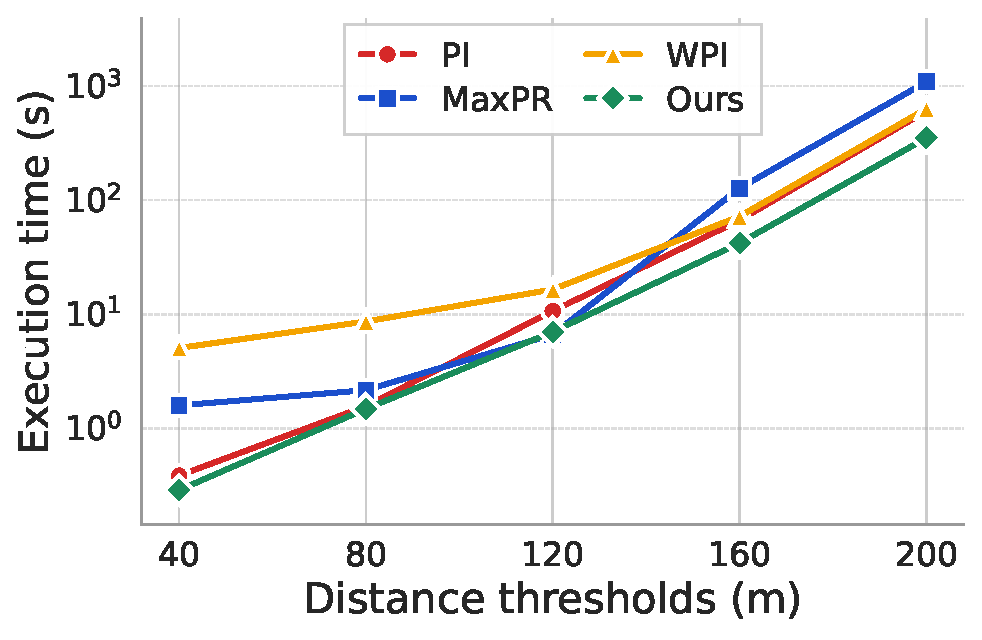
\includegraphics[width=0.32\linewidth]
  {visualization_result/LasVegas_d_Execution_time__s_.pdf}}
\hfill
\subfloat[Toronto]{%
  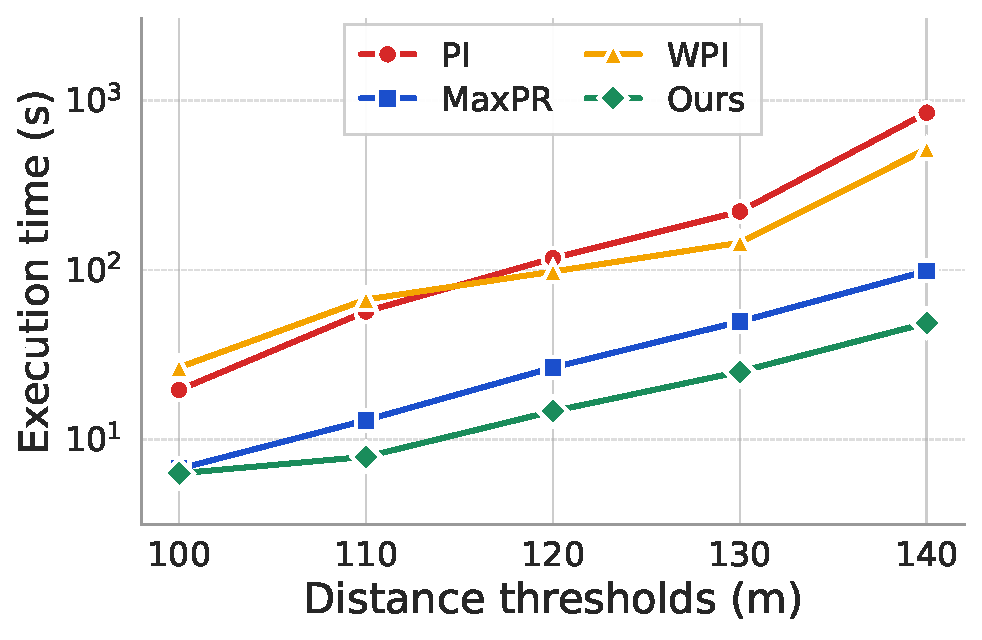
\includegraphics[width=0.32\linewidth]
  {visualization_result/Toronto_d_Execution_time__s_.pdf}}
\hfill
\subfloat[Shanghai]{%
  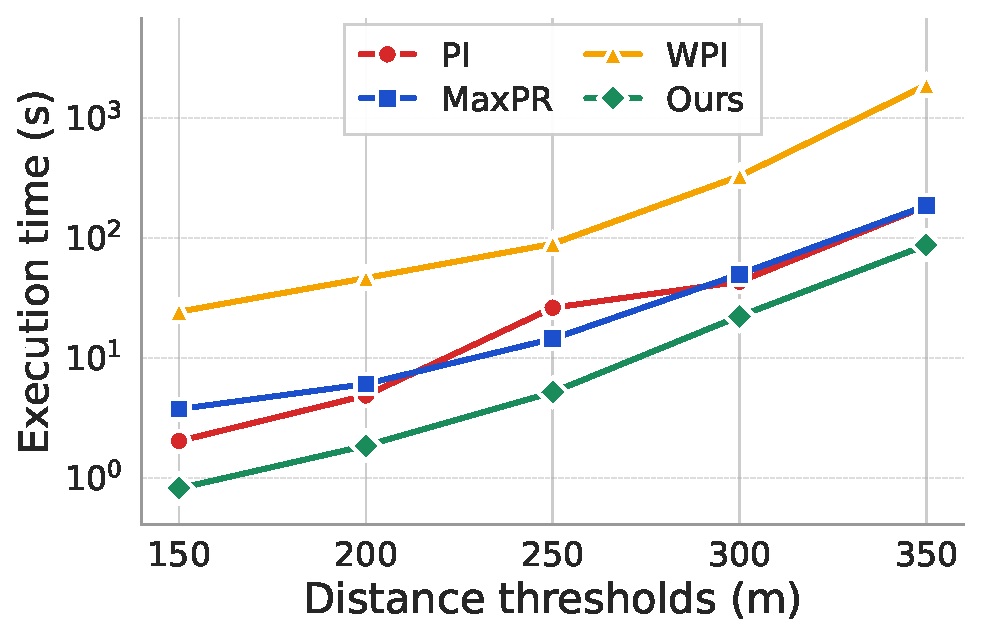
\includegraphics[width=0.32\linewidth]
  {visualization_result/Shanghai_d_Execution_time__s_.pdf}}

\par\medskip

\subfloat[Las Vegas]{%
  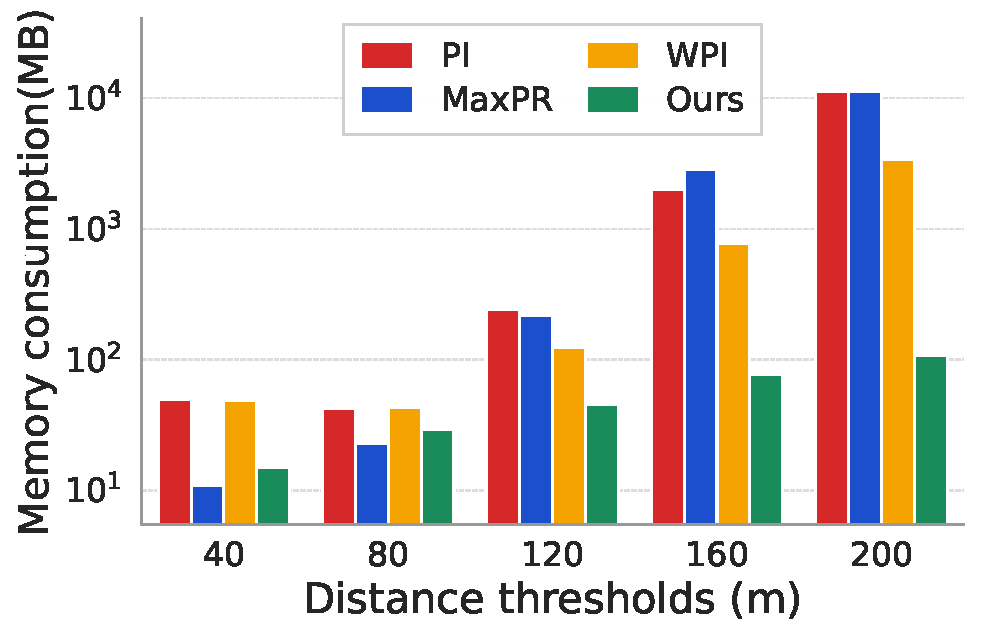
\includegraphics[width=0.32\linewidth]
  {visualization_result/LasVegas_d_Memory_consumption_MB_.pdf}}
\hfill
\subfloat[Toronto]{%
  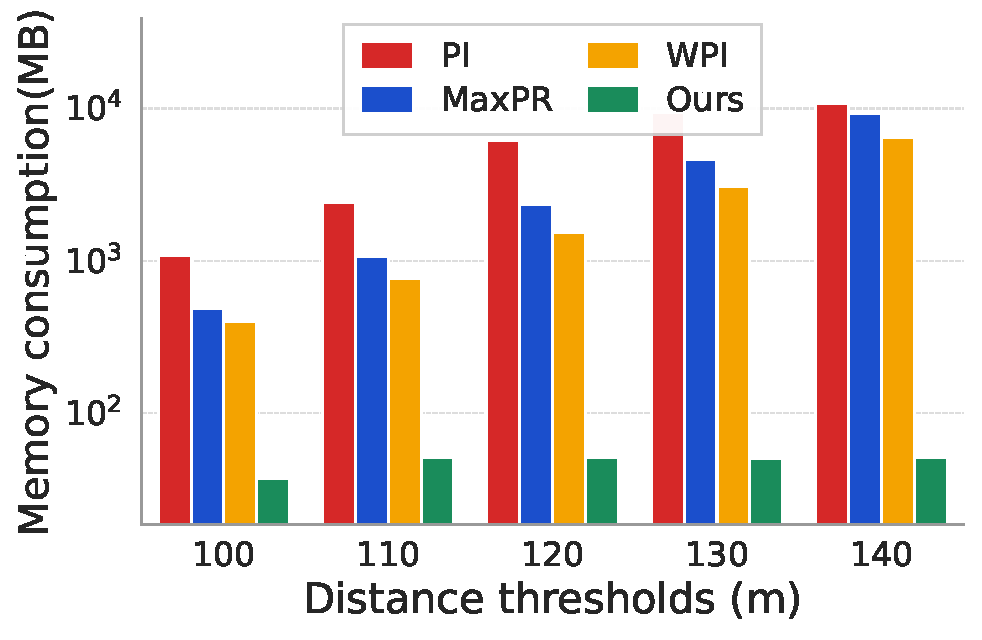
\includegraphics[width=0.32\linewidth]
  {visualization_result/Toronto_d_Memory_consumption_MB_.pdf}}
\hfill
\subfloat[Shanghai]{%
  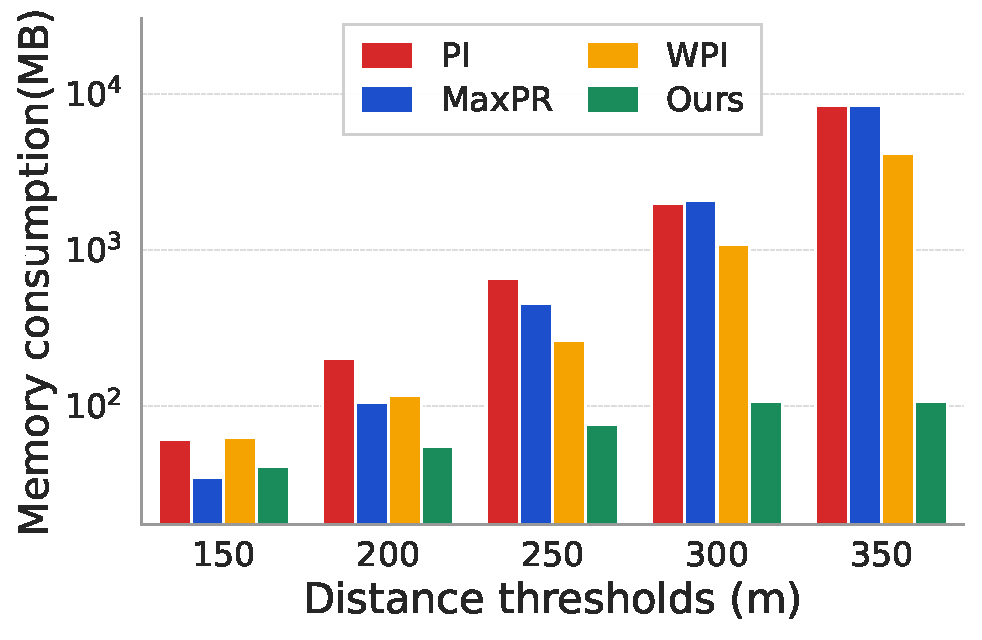
\includegraphics[width=0.32\linewidth]
  {visualization_result/Shanghai_d_Memory_consumption_MB_.pdf}}

\caption{Effect of the distance threshold $\varepsilon$ on mean runtime
(a--c) and mean peak memory (d--f)}
\label{fig:efficiency_d}
\end{figure}

\begin{figure}[tbp]
\centering
\subfloat[Las Vegas]{%
  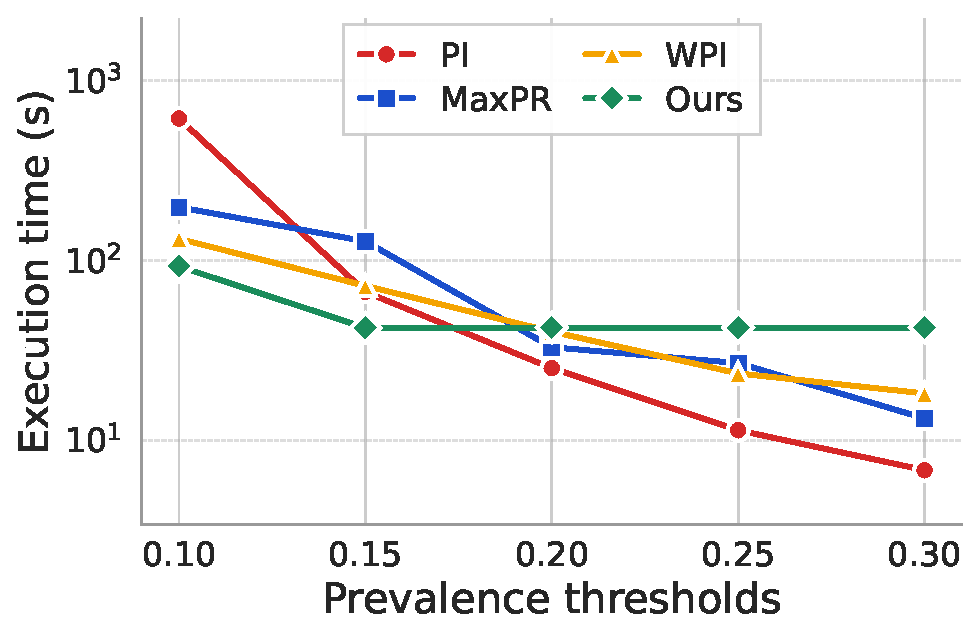
\includegraphics[width=0.32\linewidth]
  {visualization_result/LasVegas_u_Execution_time__s_.pdf}}
\hfill
\subfloat[Toronto]{%
  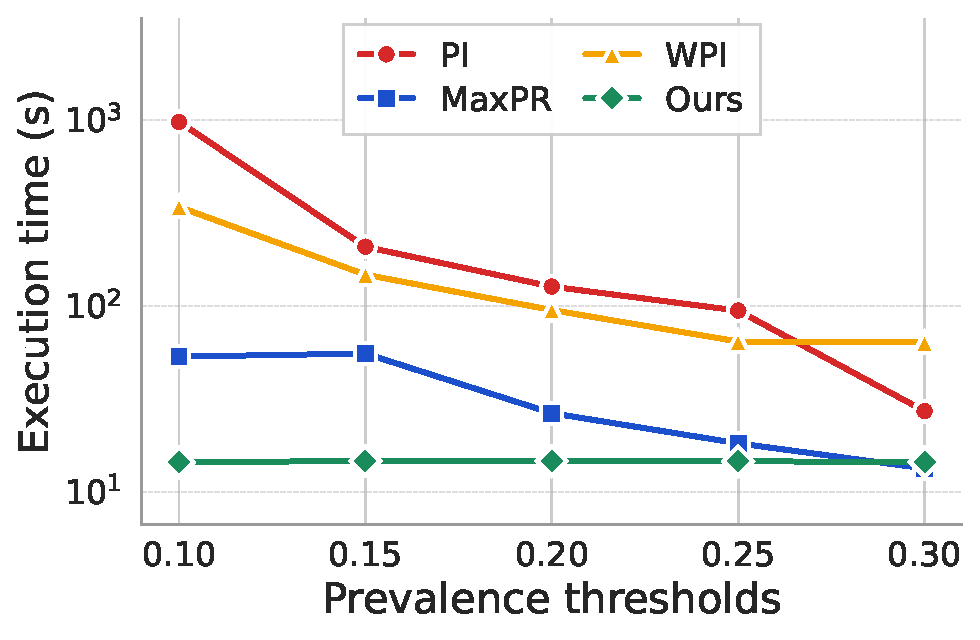
\includegraphics[width=0.32\linewidth]
  {visualization_result/Toronto_u_Execution_time__s_.pdf}}
\hfill
\subfloat[Shanghai]{%
  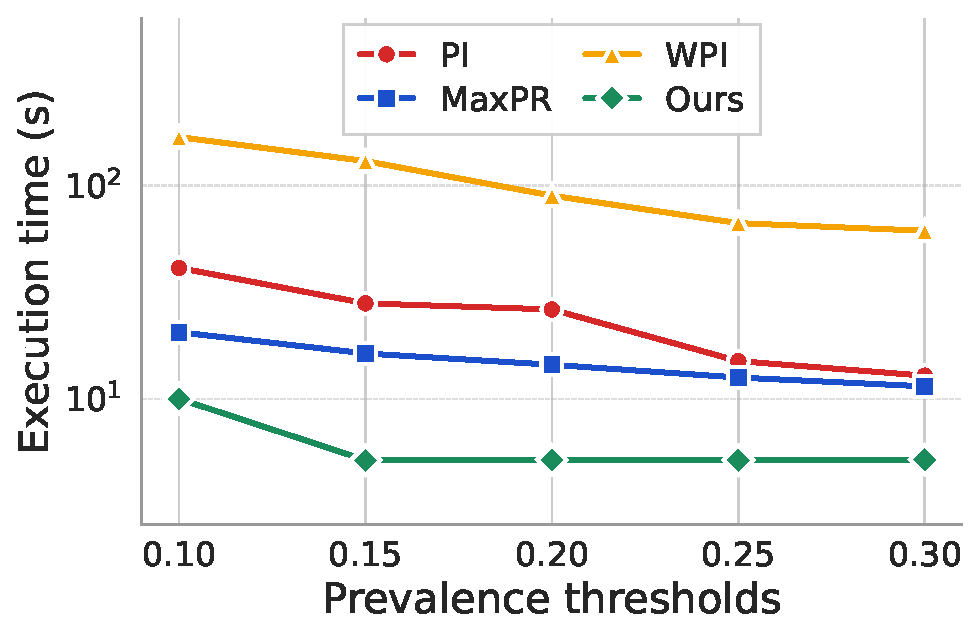
\includegraphics[width=0.32\linewidth]
  {visualization_result/Shanghai_u_Execution_time__s_.pdf}}

\par\medskip

\subfloat[Las Vegas]{%
  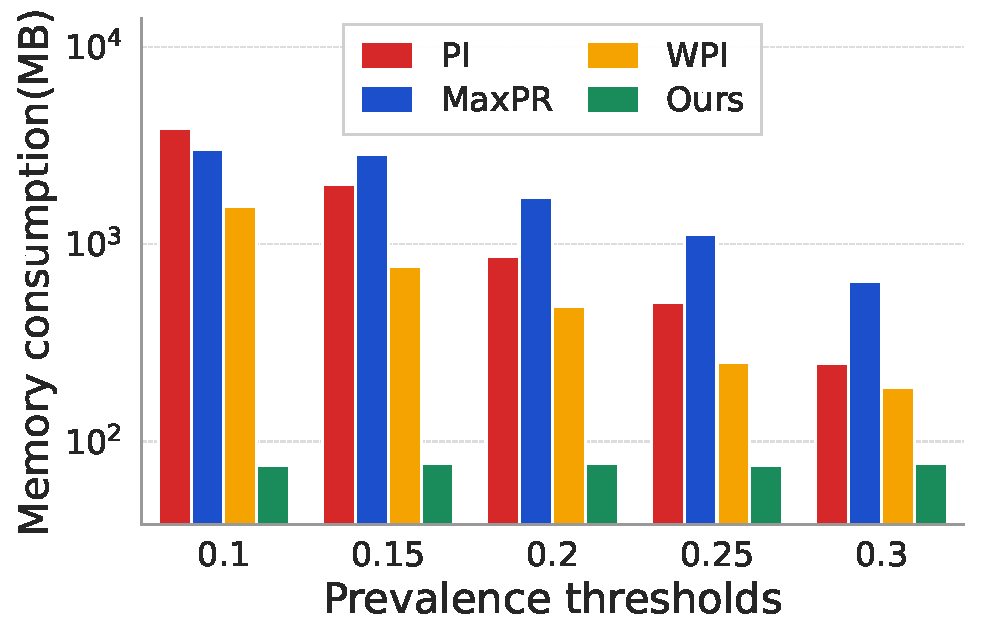
\includegraphics[width=0.32\linewidth]
  {visualization_result/LasVegas_u_Memory_consumption_MB_.pdf}}
\hfill
\subfloat[Toronto]{%
  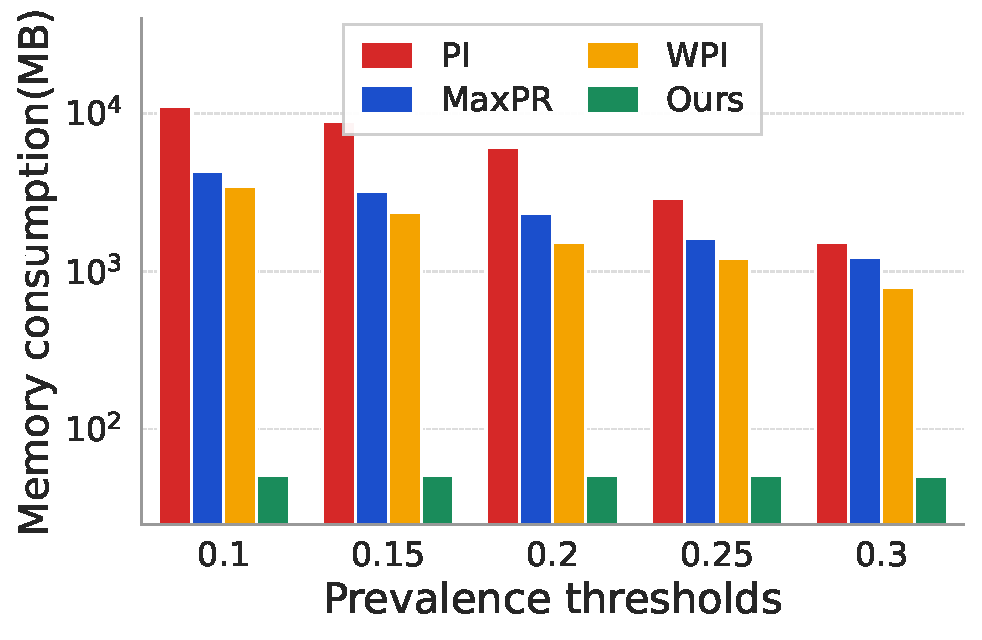
\includegraphics[width=0.32\linewidth]
  {visualization_result/Toronto_u_Memory_consumption_MB_.pdf}}
\hfill
\subfloat[Shanghai]{%
  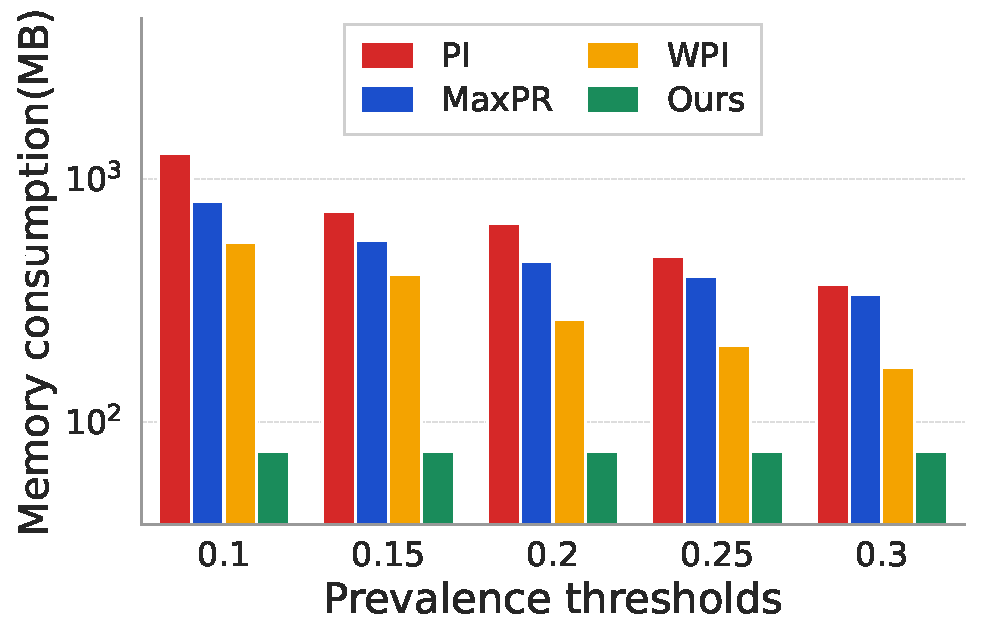
\includegraphics[width=0.32\linewidth]
  {visualization_result/Shanghai_u_Memory_consumption_MB_.pdf}}

\caption{Effect of the prevalence threshold $\minprev$ on mean runtime
(a--c) and mean peak memory (d--f)}
\label{fig:efficiency_u}
\end{figure}

\FloatBarrier

% ---------------------------------------------------------------------
\subsection{Scalability Analysis}
\label{sec:scalability}

The scalability experiment evaluates Beijing, Toronto, and Shanghai using
20\%, 40\%, 60\%, 80\%, and 100\% of their spatial instances. The prevalence
threshold is fixed at $\minprev=0.2$. The distance threshold is 250~m for
Beijing and Shanghai and 120~m for Toronto. Each plotted runtime and memory
value is averaged over four runs.

At 20--60\% of the data, a simpler baseline is occasionally faster because
its lower fixed overhead is more influential in small workloads. As the data
size increases, the runtime and memory advantages of Ours become more
apparent. In particular, the peak-memory difference is clearer from 80\%
onward, where the baselines must retain larger intermediate structures.

At 100\% of Beijing, only Ours completed within the allocated time and memory
budget. Its mean runtime was approximately 2,056.4~s, with a mean peak memory
usage of 343~MB. The baseline values at this point are missing because the
corresponding executions did not complete; they are not zero values and are
therefore excluded from numerical ranking at the 100\% setting.

\begin{figure}[tbp]
\centering
\subfloat[Beijing ($\varepsilon=250$~m)]{%
  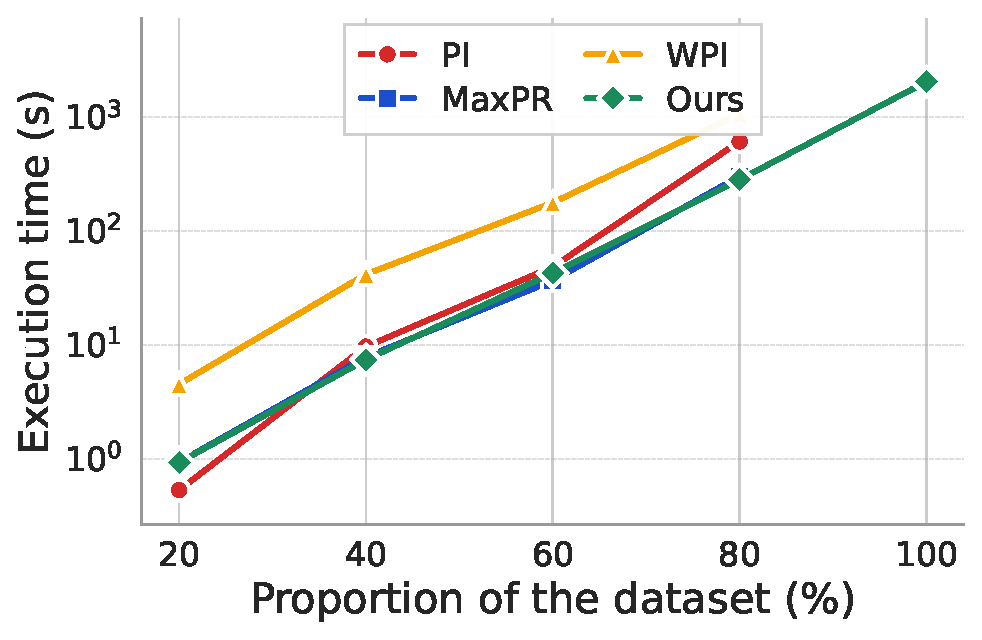
\includegraphics[width=0.32\linewidth]
  {visualization_result/Beijing__Instances_Execution_time__s_.pdf}}
\hfill
\subfloat[Toronto ($\varepsilon=120$~m)]{%
  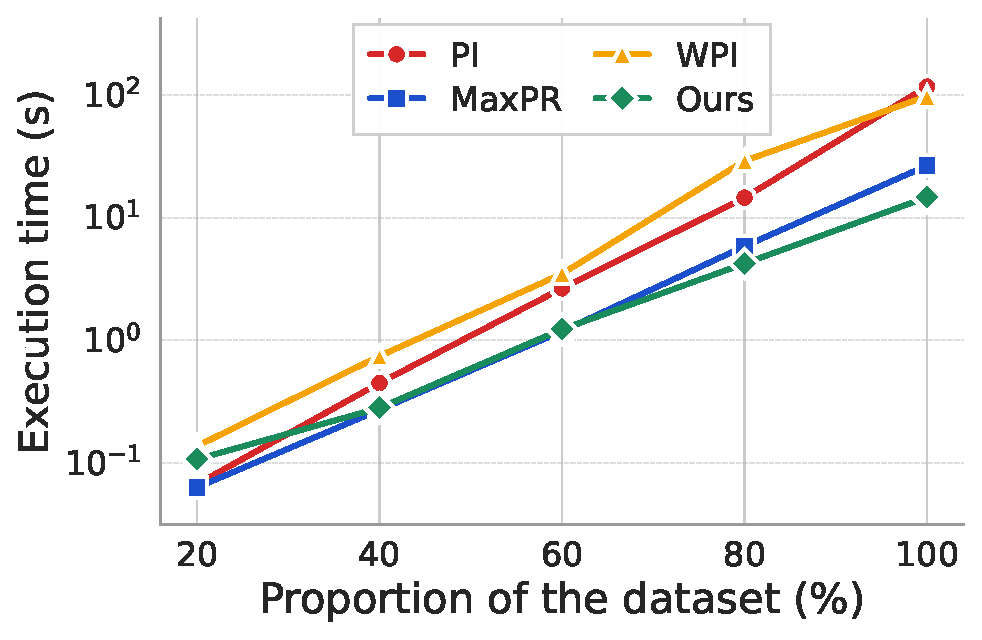
\includegraphics[width=0.32\linewidth]
  {visualization_result/Toronto__Instances_Execution_time__s_.pdf}}
\hfill
\subfloat[Shanghai ($\varepsilon=250$~m)]{%
  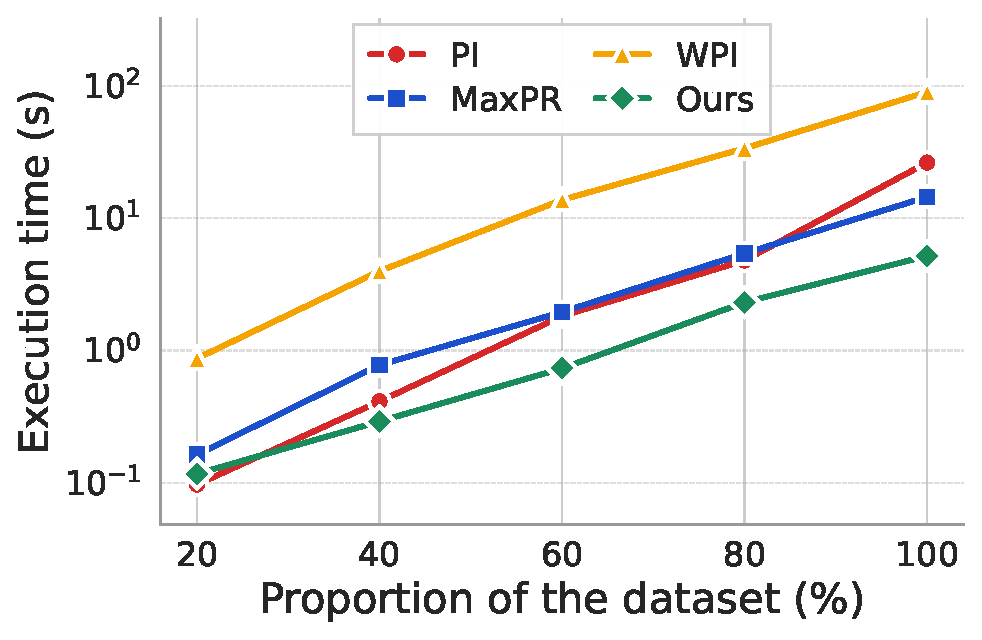
\includegraphics[width=0.32\linewidth]
  {visualization_result/Shanghai__Instances_Execution_time__s_.pdf}}

\caption{Execution-time scalability with increasing dataset size}
\label{fig:time_p}
\end{figure}

\begin{figure}[tbp]
\centering
\subfloat[Beijing ($\varepsilon=250$~m)]{%
  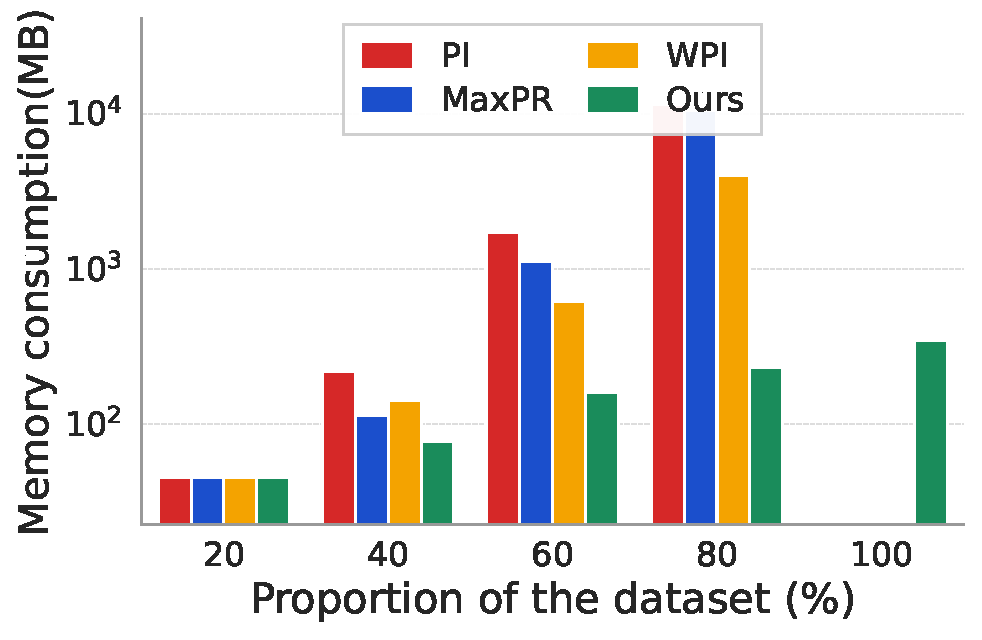
\includegraphics[width=0.32\linewidth]
  {visualization_result/Beijing__Instances_Memory_consumption_MB_.pdf}}
\hfill
\subfloat[Toronto ($\varepsilon=120$~m)]{%
  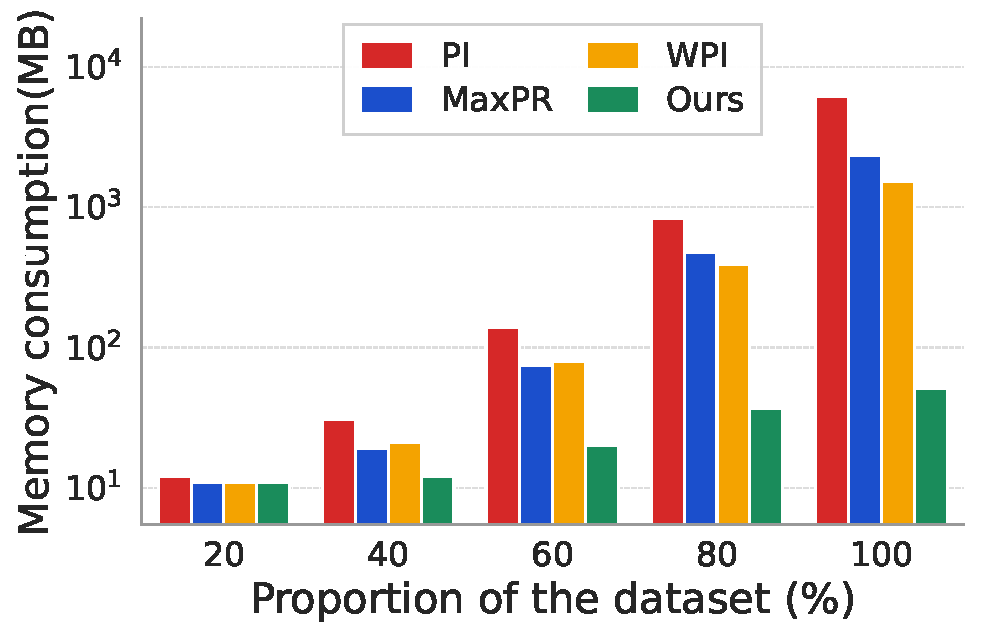
\includegraphics[width=0.32\linewidth]
  {visualization_result/Toronto__Instances_Memory_consumption_MB_.pdf}}
\hfill
\subfloat[Shanghai ($\varepsilon=250$~m)]{%
  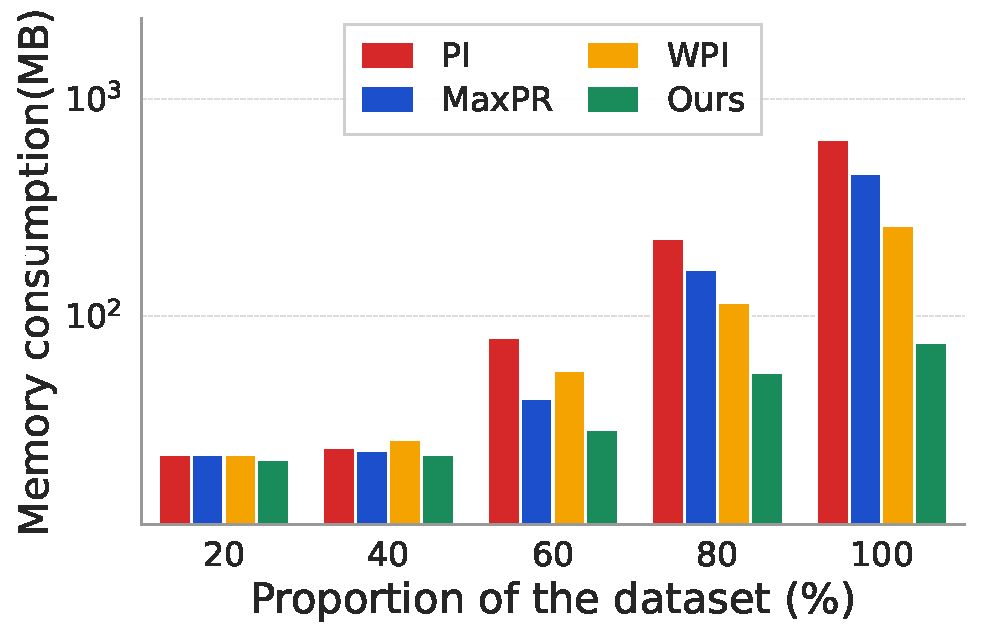
\includegraphics[width=0.32\linewidth]
  {visualization_result/Shanghai__Instances_Memory_consumption_MB_.pdf}}

\caption{Peak-memory scalability with increasing dataset size}
\label{fig:mem_p}
\end{figure}

The sampling seed used to construct the 20--80\% subsets was not retained.
Consequently, the sensitivity of the scalability curves to alternative
subsamples cannot be quantified. In addition, the figures report arithmetic
means without dispersion statistics, so they do not characterize
between-run variability.

\FloatBarrier


% ---------------------------------------------------------------------
\section{Software}\label{sec:software}

To demonstrate how the proposed mining framework can support a real
location-based application, we implemented an interactive web application, the
\emph{Co-located Spot Explorer}. The application runs the same C++ mining engine
described in Section~\ref{methodology}---the Cauchy Weighted Participation Index
($WPI_C$) together with the maximal-clique enumeration and hash-based instance
query---so that what the user sees is produced by the algorithm evaluated in this
thesis, not by a re-implementation or an approximation.

Figure~\ref{fig:software} shows the interface. The user selects one of the
downstream Yelp datasets (Philadelphia or New Orleans), sets a neighbour distance
and a popularity threshold, and runs the co-location search. The discovered
patterns are then explored spatially: clicking any point of interest on the map
highlights the venues that are co-located with it, each shown with its distance
from the selected place and its user rating. In the example, the places
co-located with a selected seafood restaurant in Philadelphia are listed on the
left, ordered by distance, while the surrounding neighbourhood and the search
radius are drawn on the map.

\begin{figure}[htbp]
  \centering
  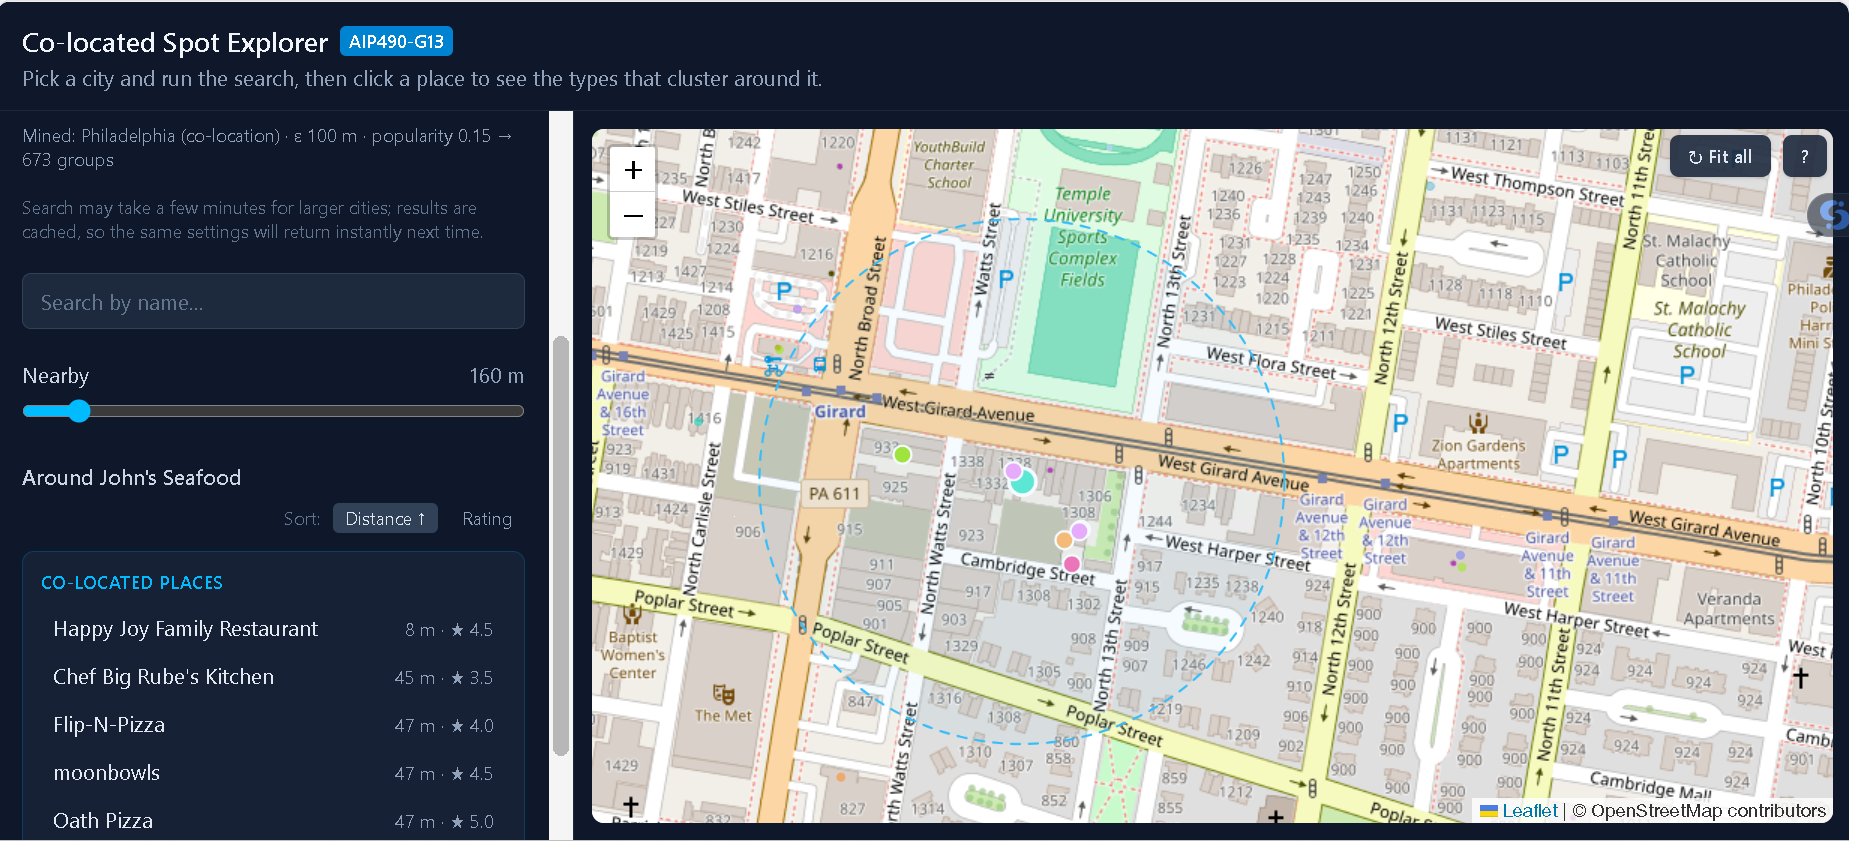
\includegraphics[width=\linewidth]{figures/software_ui.png}
  \caption{The Co-located Spot Explorer. After running the co-location search on
  a city, the user clicks a point of interest to see the categories of venues
  that co-locate around it, ranked by distance and annotated with ratings.}
  \label{fig:software}
\end{figure}

\noindent\textbf{Application to POI recommendation.} In this application, the
mined co-location patterns act as contextual signals for point-of-interest
recommendation. Rather than ranking venues in isolation, the system uses the
co-location relationships discovered by $WPI_C$ to answer a location-centred
question: given a place the user is currently interested in, which categories of
nearby venues tend to occur together with it? Because $WPI_C$ preserves patterns
that involve rare feature types, the results can surface distinctive co-located
categories that a frequency-biased measure would prune. Consistent with the
framing used throughout this thesis, the prototype is intended as a demonstration
of how spatial co-location patterns translate into a usable POI-exploration tool,
rather than as a separately evaluated recommendation model.


% ---------------------------------------------------------------------
\section{Conclusion and Future Work}\label{con}

\subsection{Conclusion}

This thesis investigated rare-feature spatial co-location pattern mining with
two main goals: improving prevalence evaluation under feature-frequency
imbalance and reducing the computational cost of the mining process.

To address the first problem, we proposed the Cauchy Weighted Participation
Index ($WPI_C$). Compared with exponential weighting, the Cauchy formulation
provides stronger adjustment under moderate imbalance while avoiding excessive
weight growth when the frequency difference becomes extreme. The experiments
show that this leads to different and more controlled prevalence decisions for
rare-feature patterns.

We then integrated $WPI_C$ into the MCR framework, which combines maximal-clique
enumeration, hash-based participating-instance retrieval, and top-down candidate
traversal. Across the evaluated datasets, MCR generally achieved lower runtime
and peak memory usage, particularly for larger or denser workloads, although
simpler methods remained competitive in several smaller configurations.

A lightweight software prototype was also developed to demonstrate how spatial
data can be used in a location-based application. It allows users to select a
location and explore nearby points of interest, but it is intended as a software
demonstration rather than an evaluated recommendation model.

Overall, the thesis combines a rarity-aware prevalence measure with an efficient
mining framework for spatial co-location discovery under imbalanced feature
distributions.


\subsection{Limitations and Future Work}

Several limitations remain. The framework is mainly evaluated on static spatial
datasets and uses a global rarity-aware weighting configuration. The evaluation
is also limited to a small number of real-world datasets, while dense
neighbourhood graphs can still make maximal-clique enumeration expensive.

Future work may therefore focus on:

\begin{itemize}

\item \textbf{Adaptive and dynamic mining.}
Investigating adaptive weighting and extending the framework to temporal,
streaming, or dynamically changing spatial data.

\item \textbf{Large-scale optimization.}
Using parallel processing, graph partitioning, improved indexing, or more
efficient candidate traversal for larger and denser datasets.

\item \textbf{Broader validation.}
Evaluating the method on additional real-world and synthetic datasets, together
with domain-specific ground truth where available.

\item \textbf{Software extensions.}
Extending the prototype with richer spatial exploration, visualisation, and
location-based functionality.

\end{itemize}

These directions would help further evaluate the scalability, adaptability, and
practical use of rare-feature spatial co-location mining.




\bibliography{arxiv}


\appendix

\end{document}